\documentclass[11pt,a4paper]{report}

\usepackage[a4paper,top=0.9in,bottom=0.9in,right=0.9in,left=1.15in]{geometry}
\usepackage{lmodern}
\usepackage{amsmath,amssymb}
\usepackage{xcolor}
\usepackage{graphicx}
\usepackage{tabularx}
\usepackage{array}
\usepackage{caption}
\usepackage{hyperref}
\usepackage{setspace}
\usepackage{tikz}
\usetikzlibrary{
  arrows.meta,
  shapes.geometric,
  shapes.multipart,
  positioning,
  fit,
  calc,
  backgrounds
}

\setstretch{1.2}
\setlength{\parskip}{4pt plus 1.5pt minus 1pt}
\setlength{\parindent}{0pt}
\renewcommand{\arraystretch}{1.28}

% Helper column type for clean ragged-right wrapping inside narrow bordered cells
\newcolumntype{L}[1]{>{\raggedright\arraybackslash}p{#1}}
\newcolumntype{Y}{>{\raggedright\arraybackslash}X}

\hypersetup{
  colorlinks=true,
  linkcolor=black,
  citecolor=black,
  urlcolor=black
}

% Unified academic TikZ styles (black-and-white LaTeX report aesthetic)
\tikzset{
  >=Stealth,
  uml line/.style={draw=black, line width=0.65pt},
  uml arrow/.style={draw=black, line width=0.65pt, ->},
  uml biarrow/.style={draw=black, line width=0.65pt, <->},
  uml dasharrow/.style={draw=black, line width=0.65pt, dashed, ->},
  uml box/.style={
    rectangle, draw=black, line width=0.65pt, fill=white,
    align=center, font=\small, inner sep=6pt, minimum height=0.9cm
  },
  uml round/.style={
    rectangle, rounded corners=4pt, draw=black, line width=0.65pt, fill=white,
    align=center, font=\small, inner sep=6pt, minimum height=0.9cm
  },
  uml oval/.style={
    ellipse, draw=black, line width=0.65pt, fill=white,
    align=center, font=\footnotesize, inner xsep=8pt, inner ysep=5pt,
    minimum width=3.8cm, minimum height=0.95cm
  },
  uml diamond/.style={
    diamond, draw=black, line width=0.65pt, fill=white,
    aspect=2.1, align=center, font=\footnotesize, inner sep=2.5pt
  },
  uml class/.style={
    rectangle split, rectangle split parts=3,
    draw=black, line width=0.65pt, fill=white,
    align=left, font=\scriptsize, inner sep=5pt,
    rectangle split part align={center, left, left}
  },
  dfd entity/.style={
    rectangle, draw=black, line width=0.75pt, fill=white,
    align=center, font=\small, inner sep=7pt, minimum width=3.0cm, minimum height=1.2cm
  },
  dfd proc/.style={
    circle, draw=black, line width=0.75pt, fill=white,
    align=center, font=\footnotesize, inner sep=3pt, minimum size=2.6cm
  },
  dfd store/.style={
    rectangle, draw=black, line width=0.75pt, fill=white,
    align=center, font=\footnotesize, inner sep=6pt,
    minimum width=4.0cm, minimum height=1.0cm
  },
  lbl/.style={
    font=\scriptsize, inner sep=2pt, align=center
  },
  uml start/.style={circle, fill=black, minimum size=8pt, inner sep=0pt},
  uml end/.style={
    circle, draw=black, line width=0.8pt, fill=white, minimum size=13pt, inner sep=0pt,
    path picture={\fill[black] (0,0) circle (3.5pt);}
  }
}

\begin{document}

% =====================================================================
% TITLE PAGE
% =====================================================================
\begin{titlepage}
\centering
\vspace*{0.6cm}
{\Large\bfseries Thapar Institute of Engineering \& Technology\par}
\vspace{0.3cm}
{\large Department of Computer Science and Engineering\par}
\vspace{1.6cm}

{\LARGE\bfseries Cloud Tunnel Gateway and Local Load Testing Platform\par}
\vspace{0.5cm}
{\large UCS503 Software Engineering Project Report\par}
{\normalsize END-Semester Evaluation\par}
\vspace{1.8cm}

{\bfseries Submitted by\par}
\vspace{0.4cm}
Jatin Bajaj \quad (1024170389)\\[4pt]
Krish Sahni \quad (1024170390)\\[4pt]
Rishabh Dutt \quad (1024170393)\\[10pt]
\vspace{0.4cm}
{\bfseries Group No.:} 3Q34\\[8pt]

\vspace{1.2cm}
{\bfseries Faculty Advisor\par}
\vspace{0.3cm}
Ms.\ Paramveer Sidhu\par

\vfill
{\normalsize Computer Science and Engineering Department\\
TIET, Patiala\\
November 2026\par}
\end{titlepage}

% =====================================================================
% PRELIMINARY PAGES (Roman Numerals)
% =====================================================================
\pagenumbering{roman}
\tableofcontents
\clearpage
\pagenumbering{arabic}

% =====================================================================
% CHAPTER 1: PROJECT SELECTION PHASE
% =====================================================================
\chapter{Project Selection Phase}

\section{Software Bid}

\textbf{Project Description}\\
Developers building backend microservices and REST APIs frequently need to benchmark how their local applications perform under high concurrent load before deploying to staging or production environments. Standard cloud load-testing tools cannot reach services running behind local firewalls or NAT on \texttt{localhost}, while local scripts mix load generation with application resources on the same process. The \textit{Cloud Tunnel Gateway and Local Load Testing Platform} solves this by hosting a persistent Netty-based binary reverse tunnel and asynchronous HTTP load-testing engine on an \textbf{AWS EC2} cloud instance, paired with a JavaFX desktop monitoring client on the developer's machine.

\textbf{Proposed Solution}\\
The platform consists of three modular Maven projects deployed across a developer workstation and an AWS EC2 instance:
\begin{itemize}
  \item \textbf{LocalLoadAgent (Java 21, JavaFX 21, Netty 4.1, Jackson):} Desktop client that saves target host/port settings, opens an outbound multiplexed binary TCP tunnel to the AWS EC2 gateway (\texttt{:9090}), forwards incoming stream frames to the local service, submits load-test configurations via REST (\texttt{:8081}), and displays live performance charts, paginated request tables, test history, and CSV exports.
  \item \textbf{CloudTunnelGateway (Java 17, Spring Boot 4.1.1, Netty 4.1, MongoDB on AWS EC2):} Cloud server hosting a Netty tunnel endpoint (\texttt{:9090}), a public TCP ingress listener (\texttt{:9100}), and a Spring WebMVC REST API (\texttt{:8081}) backed by an asynchronous \texttt{LoadTestService} (\texttt{ThreadPoolExecutor}) that persists summaries and batched per-request telemetry to MongoDB (\texttt{load\_tests} and \texttt{request\_results}).
  \item \textbf{Target Application (\texttt{student1}, Java 17, Spring Boot 4.1.1, JDBC, MySQL):} Reference local Spring Boot REST service (\texttt{GET/POST /api/users}, \texttt{GET /hello}) backed by a local MySQL \textbf{Test Database} (\texttt{student\_test\_users} on port \texttt{3306}) used to validate end-to-end cloud-to-local tunneled load testing.
\end{itemize}

\textbf{Expected Deliverables}
\begin{itemize}
  \item Persistent Netty reverse-tunnel client and AWS EC2 gateway supporting binary framing (\texttt{REGISTER}, \texttt{REGISTER\_ACK}, \texttt{OPEN\_STREAM}, \texttt{OPEN\_STREAM\_ACK}, \texttt{DATA}, \texttt{CLOSE\_STREAM}, \texttt{PING}, \texttt{PONG}).
  \item Configurable asynchronous HTTP load generator on AWS EC2 supporting custom methods, headers, query parameters, request bodies, concurrency up to 1,000, up to 100,000 requests, status-code validation, body assertions, and latency thresholds.
  \item Real-time analytics engine computing throughput (attempts/sec), failure classification, latency distributions, and P50/P95/P99 percentiles persisted in MongoDB.
  \item Interactive JavaFX desktop interface with connection management, test configuration, live execution charts, paginated request inspection, test history, and CSV export.
\end{itemize}

\textbf{Project Scope \& Expected Outcome}\\
This version focuses on single-agent TCP stream multiplexing between a local workstation and the AWS EC2 gateway, HTTP/1.1 load testing through the tunnel, MongoDB persistence, and desktop analytics visualisation. Multi-tenant authentication and distributed multi-region load injectors are outside V1 scope. The platform enables developers to stress-test local web services from AWS EC2 repeatably, pinpoint tail-latency spikes, and export structured CSV reports.

\section{Project Overview}

The \textit{Cloud Tunnel Gateway and Local Load Testing Platform} bridges a local development environment and an \textbf{AWS EC2}-hosted load-testing engine without requiring public IP exposure or manual router port forwarding. When a developer clicks \textit{Connect} in \texttt{LocalLoadAgent}, \texttt{NettyTunnelClient} opens an outbound persistent TCP channel to \texttt{TunnelGatewayServer} on AWS EC2 (\texttt{:9090}) and registers its \texttt{agentId} in \texttt{TunnelRegistry}.

Once the tunnel reports \texttt{CONNECTED}, the developer submits a load test in \texttt{LoadTestView} to \texttt{POST /api/load-tests} (\texttt{:8081}). \texttt{LoadTestService} validates the request, enqueues a \texttt{LoadTestJob} (\texttt{QUEUED} $\to$ \texttt{RUNNING}), and dispatches asynchronous HTTP requests through \texttt{PublicTcpServer} (\texttt{:9100}). Each connection receives a \texttt{streamId} in \texttt{StreamRegistry}, is multiplexed over Netty to \texttt{LocalConnectionManager}, and is forwarded to \texttt{student1} (\texttt{:8080}) backed by the MySQL Test Database. Responses return along the same stream to AWS EC2, are validated and aggregated, and are saved to MongoDB for live charting in \texttt{TestExecutionView} and browsing in \texttt{TestHistoryView}.

% =====================================================================
% CHAPTER 2: ANALYSIS PHASE
% =====================================================================
\chapter{Analysis Phase}

\section{Use Cases}

\subsection{Use-Case Diagrams}

Figure~\ref{fig:usecase} models runtime interactions between \textit{Developer / Tester}, \textit{Local Target App (\texttt{student1})}, and \textit{MongoDB Database}. Mandatory shared behaviours are linked via $\ll$include$\gg$ arrows, while optional CSV export extends analytics monitoring via $\ll$extend$\gg$.

\begin{figure}[!htbp]
\centering
\resizebox{\linewidth}{!}{%
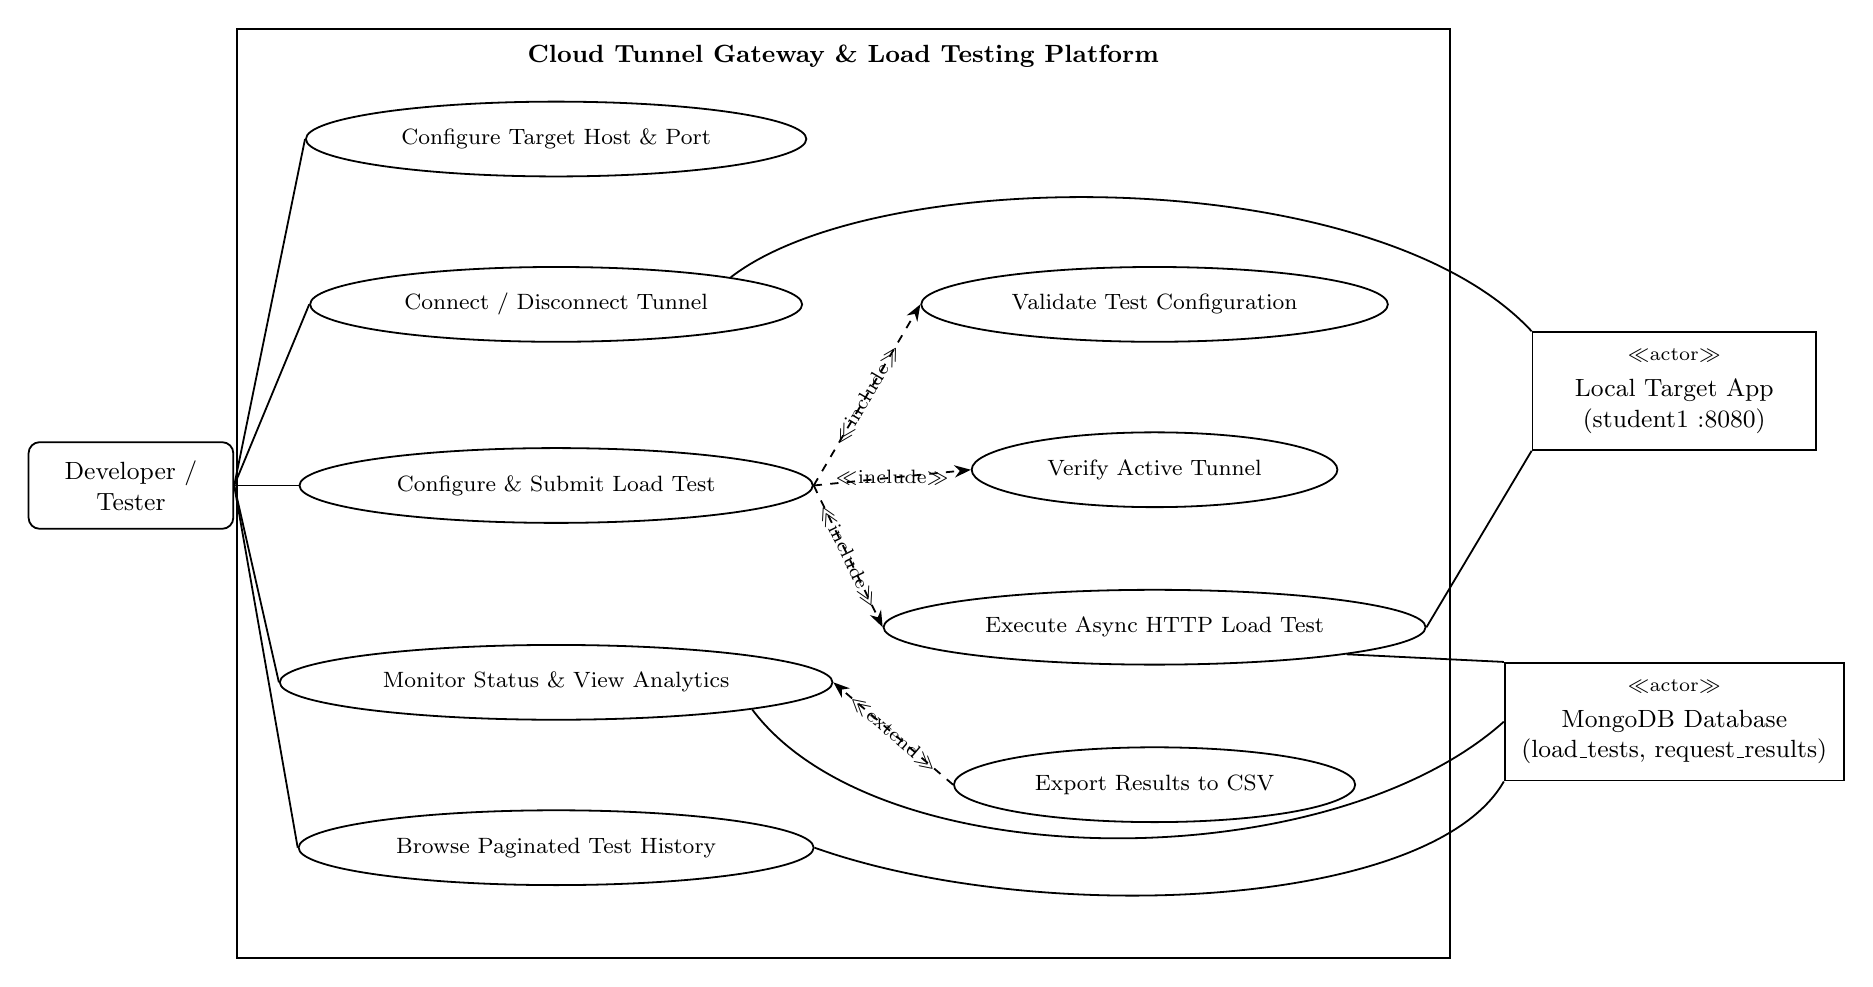
\begin{tikzpicture}

  % Primary Actor (Left)
  \node[uml round, minimum width=2.6cm, minimum height=1.1cm] (dev) at (0, 0) {Developer /\\Tester};

  % Left column Use Cases
  \node[uml oval] (uc1) at (5.4,  4.4) {Configure Target Host \& Port};
  \node[uml oval] (uc2) at (5.4,  2.3) {Connect / Disconnect Tunnel};
  \node[uml oval] (uc3) at (5.4,  0.0) {Configure \& Submit Load Test};
  \node[uml oval] (uc4) at (5.4, -2.5) {Monitor Status \& View Analytics};
  \node[uml oval] (uc5) at (5.4, -4.6) {Browse Paginated Test History};

  % Right column Included / Extended Use Cases (wide horizontal gap)
  \node[uml oval] (uc6) at (13.0,  2.3) {Validate Test Configuration};
  \node[uml oval] (uc7) at (13.0,  0.2) {Verify Active Tunnel};
  \node[uml oval] (uc8) at (13.0, -1.8) {Execute Async HTTP Load Test};
  \node[uml oval] (uc9) at (13.0, -3.8) {Export Results to CSV};

  % System Boundary Box
  \begin{scope}[on background layer]
    \node[draw=black, line width=0.8pt, fill=white,
          fit=(uc1)(uc5)(uc6)(uc9), inner xsep=22pt, inner ysep=26pt,
          label={[font=\bfseries\small, yshift=-18pt]north:Cloud Tunnel Gateway \& Load Testing Platform}] (sys) {};
  \end{scope}

  % Secondary Actors (Right, outside boundary with generous gap)
  \node[uml box, minimum width=3.6cm] (target) at (19.6,  1.2) {\scriptsize$\ll$actor$\gg$\\[2pt]\small Local Target App\\(student1 :8080)};
  \node[uml box, minimum width=3.6cm] (mongo)  at (19.6, -3.0) {\scriptsize$\ll$actor$\gg$\\[2pt]\small MongoDB Database\\(load\_tests, request\_results)};

  % Primary Actor associations
  \draw[uml line] (dev.east) -- (uc1.west);
  \draw[uml line] (dev.east) -- (uc2.west);
  \draw[uml line] (dev.east) -- (uc3.west);
  \draw[uml line] (dev.east) -- (uc4.west);
  \draw[uml line] (dev.east) -- (uc5.west);

  % <<include>> arrows (base -> included)
  \draw[uml dasharrow] (uc3.east) -- node[lbl, sloped, pos=0.5] {$\ll$include$\gg$} (uc6.west);
  \draw[uml dasharrow] (uc3.east) -- node[lbl, pos=0.5] {$\ll$include$\gg$} (uc7.west);
  \draw[uml dasharrow] (uc3.east) -- node[lbl, sloped, pos=0.5] {$\ll$include$\gg$} (uc8.west);

  % <<extend>> arrow (extending -> base)
  \draw[uml dasharrow] (uc9.west) -- node[lbl, sloped, pos=0.5] {$\ll$extend$\gg$} (uc4.east);

  % Secondary Actor associations (routed cleanly outside ovals)
  \draw[uml line] (uc2.north east) .. controls (9.5, 4.1) and (15.8, 4.1) .. (target.north west);
  \draw[uml line] (uc8.east) -- (target.south west);
  \draw[uml line] (uc8.south east) -- (mongo.north west);
  \draw[uml line] (uc4.south east) .. controls (9.5, -5.0) and (15.2, -5.0) .. (mongo.west);
  \draw[uml line] (uc5.east) .. controls (11.5, -5.6) and (16.5, -5.4) .. (mongo.south west);

\end{tikzpicture}%
}
\caption{Use-Case Diagram for the Cloud Tunnel Gateway and Load Testing Platform.}
\label{fig:usecase}
\end{figure}

\begin{table}[!htbp]
\centering
\small
\caption{Summary of System Use Cases}
\label{tab:usecases}
\begin{tabularx}{\linewidth}{|L{1.2cm}|L{4.0cm}|Y|}
\hline
\textbf{ID} & \textbf{Use Case} & \textbf{Description} \\
\hline
UC-01 & Configure Target Host \& Port & Persists local target host and port in Java \texttt{Preferences} via \texttt{TargetConfigurationStore}. \\
\hline
UC-02 & Connect / Disconnect Tunnel & Opens or closes the persistent Netty binary tunnel to AWS EC2 (\texttt{:9090}) and updates \texttt{ConnectionStatus}. \\
\hline
UC-03 & Configure \& Submit Load Test & Captures URL, method, request count, concurrency, timeout, headers, body, and assertions, then calls \texttt{POST /api/load-tests}. \\
\hline
UC-04 & Validate Test Configuration & Checks port bounds, request/concurrency caps, HTTP status code range (100--599), and payload limits. \\
\hline
UC-05 & Verify Active Tunnel & Confirms \texttt{ConnectionStatus.CONNECTED} before permitting test submission. \\
\hline
UC-06 & Execute Async HTTP Load Test & Dispatches concurrent HTTP requests on AWS EC2 via \texttt{PublicTcpServer} (\texttt{:9100}) through the tunnel to \texttt{student1} (\texttt{:8080}) and persists results to MongoDB. \\
\hline
UC-07 & Monitor Status \& View Analytics & Polls \texttt{GET /api/load-tests/\{testId\}}, fetches summary metrics and paginated request rows, and renders Pie, Throughput, Latency, and Scatter charts. \\
\hline
UC-08 & Export Results to CSV & Writes summary KPIs, throughput buckets, latency distribution, and all request details to a local CSV file. \\
\hline
UC-09 & Browse Paginated Test History & Queries \texttt{GET /api/load-tests/history} and opens historical runs on double-click. \\
\hline
\end{tabularx}
\end{table}

\subsection{Use Case Templates}

\textbf{Use Case ID:} UC-03 / UC-06 \quad \textbf{Name:} Configure, Submit, and Execute Tunneled Load Test\\
\textbf{Primary Actor:} Developer / Tester \quad \textbf{Secondary Actors:} Local Target App (\texttt{student1}), MongoDB Database\\
\textbf{Preconditions:} \texttt{CloudTunnelGateway} is running on AWS EC2 (\texttt{:8081}, \texttt{:9090}, \texttt{:9100}) with MongoDB reachable; \texttt{student1} (\texttt{:8080}) is connected to the MySQL Test Database (\texttt{:3306}); \texttt{LocalLoadAgent} reports \texttt{CONNECTED}.\\
\textbf{Trigger:} The developer clicks \textit{Start Load Test} in \texttt{LoadTestView}.\\
\textbf{Main Flow:}
\begin{enumerate}
  \item \texttt{LoadTestView} validates the active tunnel and configuration fields; \texttt{LoadTestApiClient} posts JSON to \texttt{POST /api/load-tests} on AWS EC2.
  \item \texttt{LoadTestService.startTest()} validates limits, enqueues \texttt{LoadTestJob} (\texttt{QUEUED}), persists the initial \texttt{LoadTestDocument}, and returns \texttt{testId}.
  \item A worker marks the job \texttt{RUNNING} and dispatches concurrent HTTP requests via \texttt{PublicTcpServer} (\texttt{:9100}) through Netty \texttt{OPEN\_STREAM}/\texttt{DATA} frames to \texttt{LocalConnectionManager} and \texttt{student1} (\texttt{:8080}).
  \item Responses return to AWS EC2, are validated against status, body, and latency assertions, and failures are classified by \texttt{FailureType}.
  \item On completion, \texttt{LoadTestService} aggregates RPS, P50/P95/P99 latencies, and timelines, persists \texttt{load\_tests} and batched \texttt{request\_results} to MongoDB, and marks the job \texttt{COMPLETED}.
  \item \texttt{TestExecutionView} detects \texttt{COMPLETED} via polling and renders all charts and paginated request rows.
\end{enumerate}
\textbf{Alternative Flows:} Disconnected tunnel blocks submission with an error banner; invalid configuration returns HTTP \texttt{400}; runtime/DB failures mark the job \texttt{FAILED} and display the error in \texttt{TestExecutionView}.\\
\textbf{Postconditions:} Test summary and per-request telemetry are persisted in MongoDB and accessible in \texttt{TestExecutionView} and \texttt{TestHistoryView}.

\section{Activity Diagram and Swimlane Diagrams}

Figure~\ref{fig:activity} illustrates tunnel setup, validation, parallel AWS EC2 load execution and UI status polling (fork/join), and optional CSV export. Figure~\ref{fig:swimlane} partitions the tunneled execution across four responsibility lanes.

\begin{figure}[!htbp]
\centering
\resizebox{0.82\linewidth}{!}{%
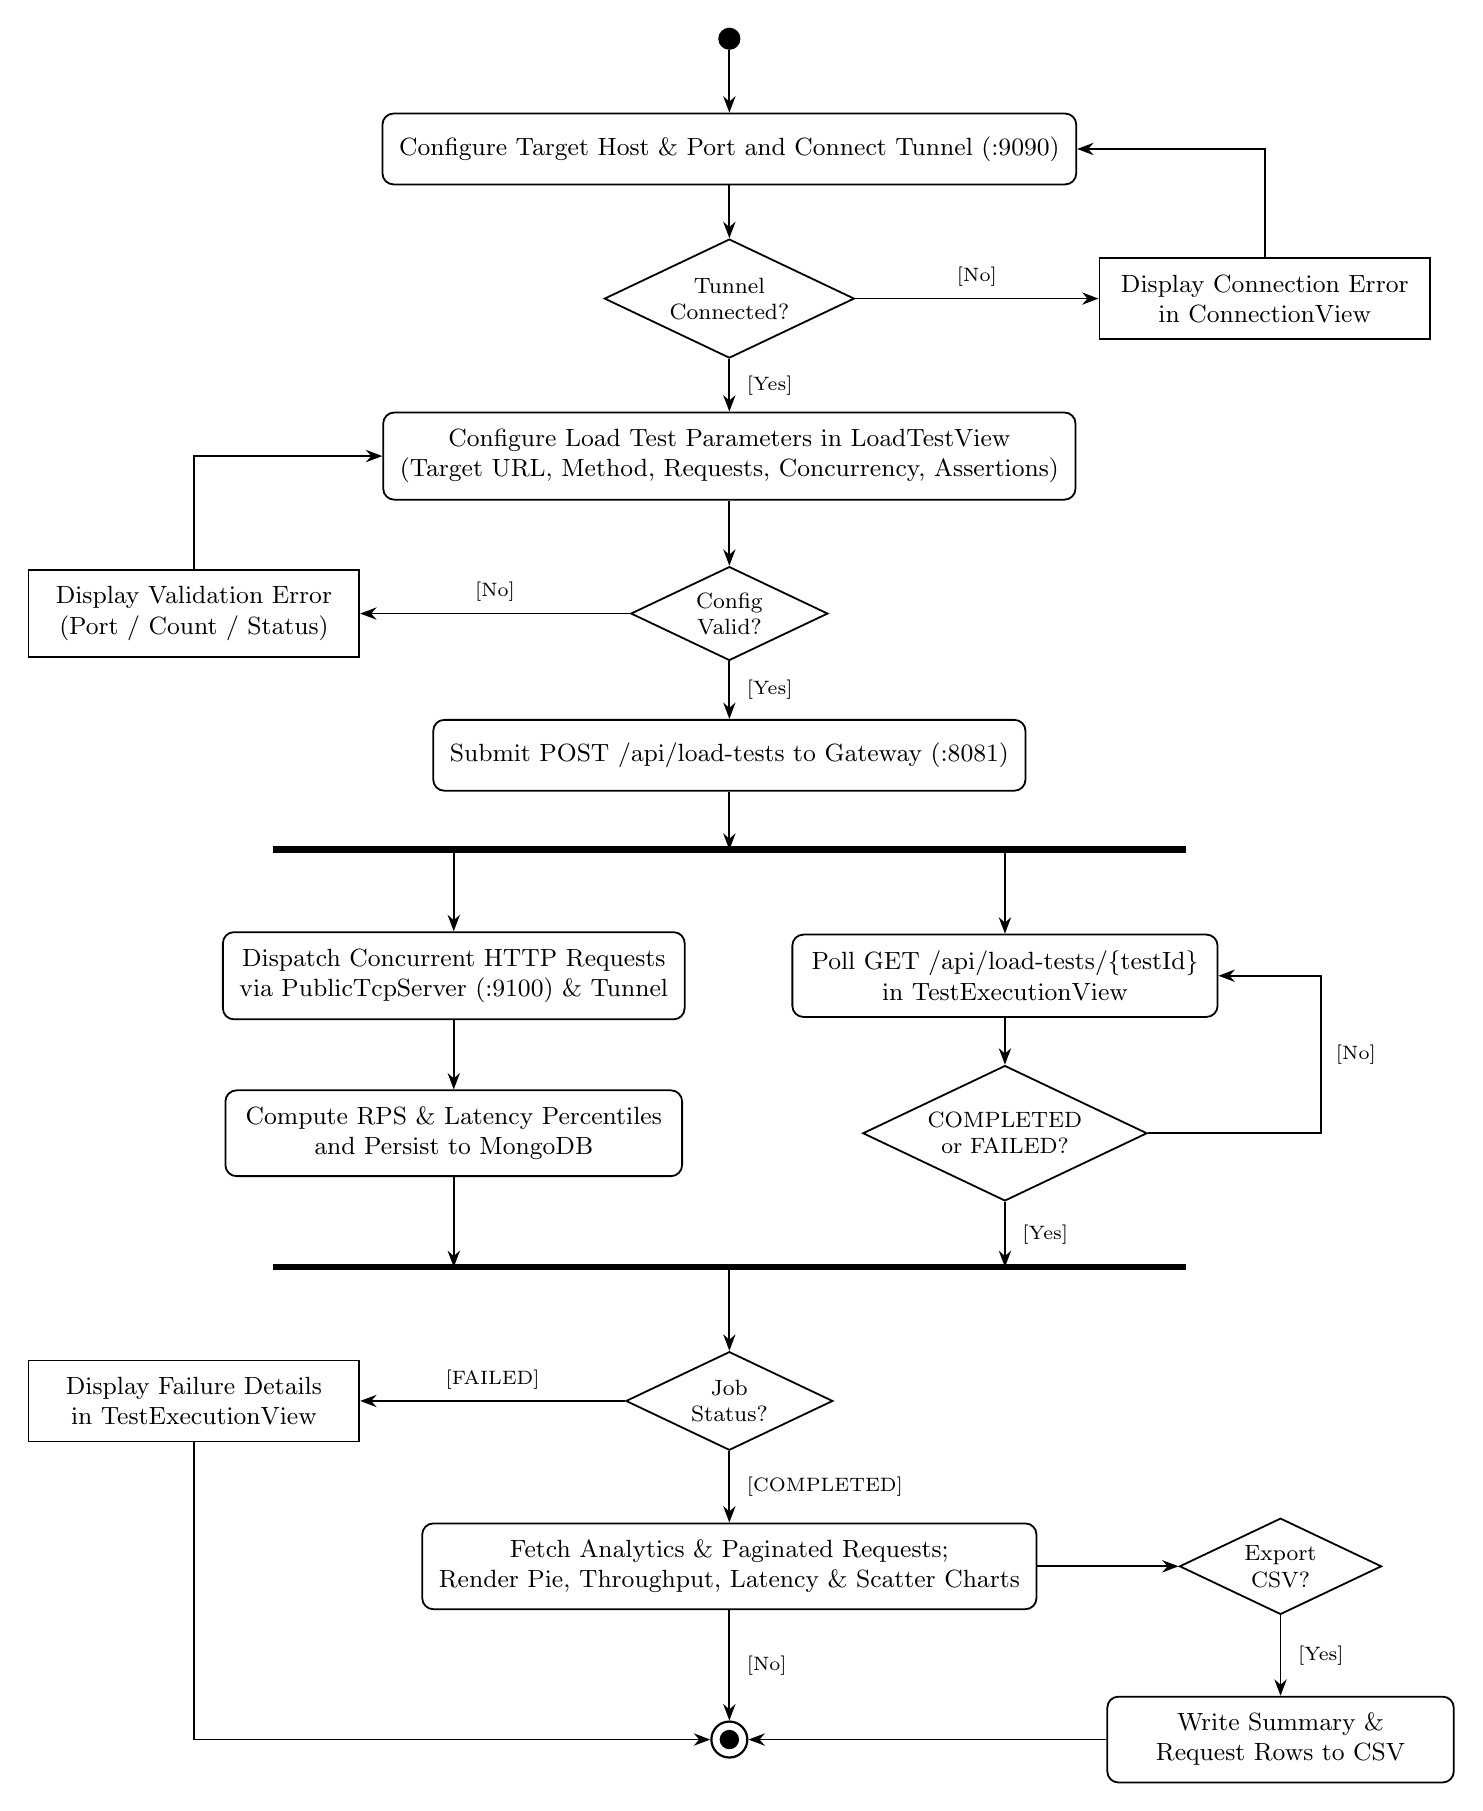
\begin{tikzpicture}

  \node[uml start] (s) at (0, 0) {};
  \node[uml round, minimum width=7.4cm] (a1) at (0, -1.4) {Configure Target Host \& Port and Connect Tunnel (:9090)};
  \node[uml diamond] (d1) at (0, -3.3) {Tunnel\\Connected?};
  \node[uml box, minimum width=4.2cm] (err1) at (6.8, -3.3) {Display Connection Error\\in ConnectionView};

  \node[uml round, minimum width=7.4cm] (a2) at (0, -5.3) {Configure Load Test Parameters in LoadTestView\\(Target URL, Method, Requests, Concurrency, Assertions)};
  \node[uml diamond] (d2) at (0, -7.3) {Config\\Valid?};
  \node[uml box, minimum width=4.2cm] (err2) at (-6.8, -7.3) {Display Validation Error\\(Port / Count / Status)};

  \node[uml round, minimum width=6.8cm] (a3) at (0, -9.1) {Submit POST /api/load-tests to Gateway (:8081)};

  % Fork bar
  \draw[black, line width=2.4pt] (-5.8, -10.3) -- (5.8, -10.3);
  \coordinate (forkC) at (0, -10.3);
  \coordinate (forkL) at (-3.5, -10.3);
  \coordinate (forkR) at (3.5, -10.3);

  % Left parallel branch (Gateway)
  \node[uml round, minimum width=5.8cm] (p1) at (-3.5, -11.9) {Dispatch Concurrent HTTP Requests\\via PublicTcpServer (:9100) \& Tunnel};
  \node[uml round, minimum width=5.8cm] (p2) at (-3.5, -13.9) {Compute RPS \& Latency Percentiles\\and Persist to MongoDB};

  % Right parallel branch (UI Polling)
  \node[uml round, minimum width=5.4cm] (q1) at (3.5, -11.9) {Poll GET /api/load-tests/\{testId\}\\in TestExecutionView};
  \node[uml diamond] (dq) at (3.5, -13.9) {COMPLETED\\or FAILED?};

  % Join bar
  \draw[black, line width=2.4pt] (-5.8, -15.6) -- (5.8, -15.6);
  \coordinate (joinC) at (0, -15.6);
  \coordinate (joinL) at (-3.5, -15.6);
  \coordinate (joinR) at (3.5, -15.6);

  \node[uml diamond] (d3) at (0, -17.3) {Job\\Status?};
  \node[uml box, minimum width=4.2cm] (err3) at (-6.8, -17.3) {Display Failure Details\\in TestExecutionView};

  \node[uml round, minimum width=6.8cm] (a4) at (0, -19.4) {Fetch Analytics \& Paginated Requests;\\Render Pie, Throughput, Latency \& Scatter Charts};
  \node[uml diamond] (d4) at (7.0, -19.4) {Export\\CSV?};
  \node[uml round, minimum width=4.4cm] (csv) at (7.0, -21.6) {Write Summary \&\\Request Rows to CSV};
  \node[uml end] (e) at (0, -21.6) {};

  % Arrows (all routed cleanly outside shapes)
  \draw[uml arrow] (s) -- (a1);
  \draw[uml arrow] (a1) -- (d1);
  \draw[uml arrow] (d1.east) -- node[lbl, above=2pt] {[No]} (err1.west);
  \draw[uml arrow] (err1.north) |- (a1.east);
  \draw[uml arrow] (d1.south) -- node[lbl, right=4pt] {[Yes]} (a2.north);
  \draw[uml arrow] (a2) -- (d2);
  \draw[uml arrow] (d2.west) -- node[lbl, above=2pt] {[No]} (err2.east);
  \draw[uml arrow] (err2.north) |- (a2.west);
  \draw[uml arrow] (d2.south) -- node[lbl, right=4pt] {[Yes]} (a3.north);
  \draw[uml arrow] (a3.south) -- (forkC);

  % Parallel branches
  \draw[uml arrow] (forkL) -- (p1.north);
  \draw[uml arrow] (p1.south) -- (p2.north);
  \draw[uml arrow] (p2.south) -- (joinL);

  \draw[uml arrow] (forkR) -- (q1.north);
  \draw[uml arrow] (q1.south) -- (dq.north);
  \draw[uml arrow] (dq.east) -- ++(2.2, 0) |- node[lbl, pos=0.25, right=3pt] {[No]} (q1.east);
  \draw[uml arrow] (dq.south) -- node[lbl, right=4pt] {[Yes]} (joinR);

  % Post-join
  \draw[uml arrow] (joinC) -- (d3.north);
  \draw[uml arrow] (d3.west) -- node[lbl, above=2pt] {[FAILED]} (err3.east);
  \draw[uml arrow] (err3.south) |- (e.west);
  \draw[uml arrow] (d3.south) -- node[lbl, right=4pt] {[COMPLETED]} (a4.north);
  \draw[uml arrow] (a4.east) -- (d4.west);
  \draw[uml arrow] (d4.south) -- node[lbl, right=4pt] {[Yes]} (csv.north);
  \draw[uml arrow] (csv.west) -- (e.east);
  \draw[uml arrow] (a4.south) -- node[lbl, right=4pt] {[No]} (e.north);

\end{tikzpicture}%
}
\caption{Activity Diagram for Load Test Configuration, Parallel Execution, Polling, and Analytics.}
\label{fig:activity}
\end{figure}

\begin{figure}[!htbp]
\centering
\resizebox{0.92\linewidth}{!}{%
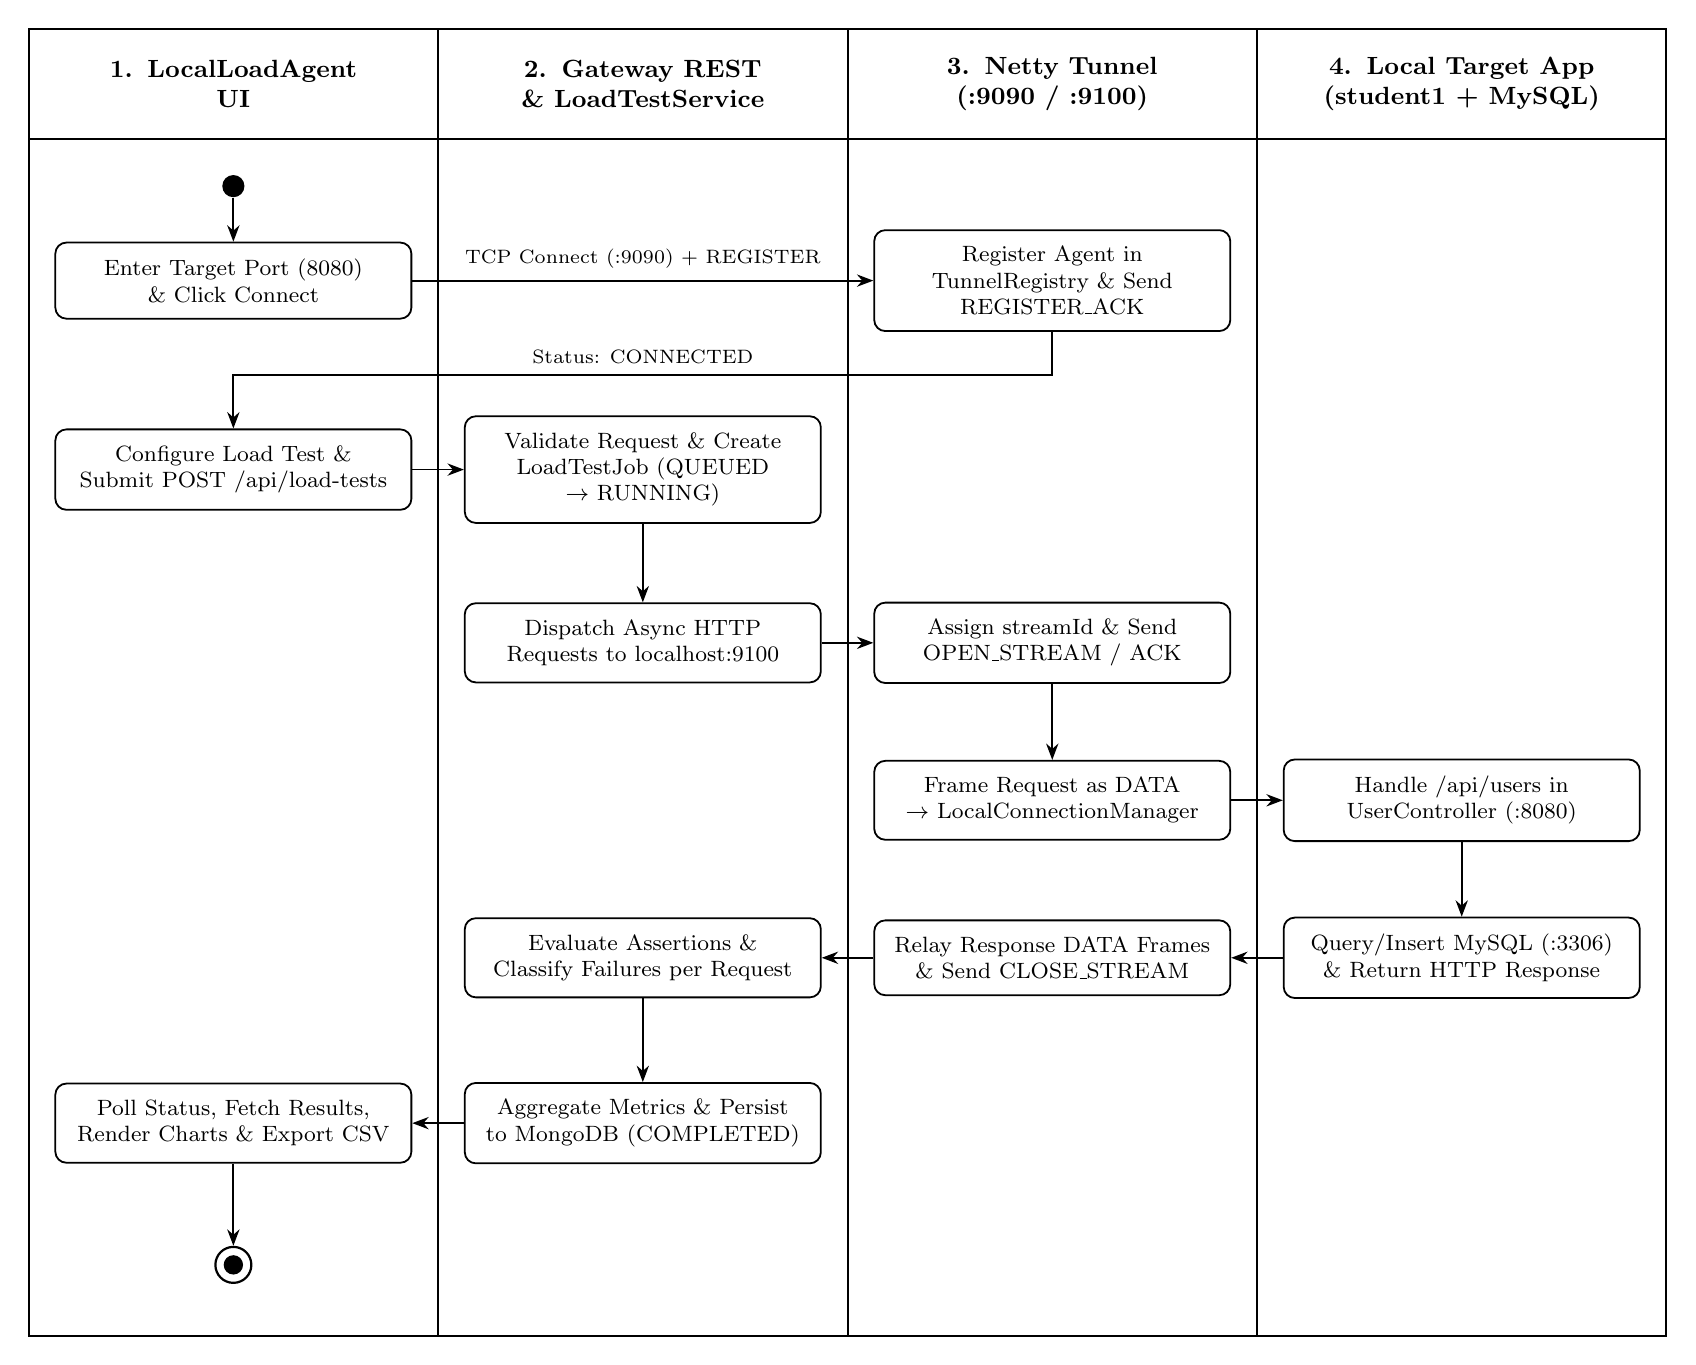
\begin{tikzpicture}

  % 4 Wide Swimlanes (each 5.2cm wide, total 20.8cm; 2-line headers so zero overflow)
  \def\lw{5.2}
  \def\topY{0}
  \def\hdrY{-1.4}
  \def\botY{-16.6}

  \foreach \i/\title in {
    0/{1. LocalLoadAgent\\UI},
    1/{2. Gateway REST\\\& LoadTestService},
    2/{3. Netty Tunnel\\(:9090 / :9100)},
    3/{4. Local Target App\\(student1 + MySQL)}
  }{
    \draw[black, line width=0.7pt] (\i*\lw, \topY) rectangle ({(\i+1)*\lw}, \botY);
    \draw[black, line width=0.7pt] (\i*\lw, \topY) rectangle ({(\i+1)*\lw}, \hdrY);
    \node[font=\bfseries\small, align=center, text width=4.6cm] at ({(\i+0.5)*\lw}, -0.7) {\title};
  }

  % Lane centers: 2.6, 7.8, 13.0, 18.2
  \node[uml start] (st) at (2.6, -2.0) {};
  \node[uml round, text width=4.1cm, font=\footnotesize] (n1) at (2.6, -3.2) {Enter Target Port (8080)\\\& Click Connect};
  \node[uml round, text width=4.1cm, font=\footnotesize] (n2) at (13.0, -3.2) {Register Agent in\\TunnelRegistry \& Send\\REGISTER\_ACK};
  \node[uml round, text width=4.1cm, font=\footnotesize] (n3) at (2.6, -5.6) {Configure Load Test \&\\Submit POST /api/load-tests};
  \node[uml round, text width=4.1cm, font=\footnotesize] (n4) at (7.8, -5.6) {Validate Request \& Create\\LoadTestJob (QUEUED $\to$ RUNNING)};
  \node[uml round, text width=4.1cm, font=\footnotesize] (n5) at (7.8, -7.8) {Dispatch Async HTTP\\Requests to localhost:9100};
  \node[uml round, text width=4.1cm, font=\footnotesize] (n6) at (13.0, -7.8) {Assign streamId \& Send\\OPEN\_STREAM / ACK};
  \node[uml round, text width=4.1cm, font=\footnotesize] (n7) at (13.0, -9.8) {Frame Request as DATA\\$\to$ LocalConnectionManager};
  \node[uml round, text width=4.1cm, font=\footnotesize] (n8) at (18.2, -9.8) {Handle /api/users in\\UserController (:8080)};
  \node[uml round, text width=4.1cm, font=\footnotesize] (n9) at (18.2, -11.8) {Query/Insert MySQL (:3306)\\\& Return HTTP Response};
  \node[uml round, text width=4.1cm, font=\footnotesize] (n10) at (13.0, -11.8) {Relay Response DATA Frames\\\& Send CLOSE\_STREAM};
  \node[uml round, text width=4.1cm, font=\footnotesize] (n11) at (7.8, -11.8) {Evaluate Assertions \&\\Classify Failures per Request};
  \node[uml round, text width=4.1cm, font=\footnotesize] (n12) at (7.8, -13.9) {Aggregate Metrics \& Persist\\to MongoDB (COMPLETED)};
  \node[uml round, text width=4.1cm, font=\footnotesize] (n13) at (2.6, -13.9) {Poll Status, Fetch Results,\\Render Charts \& Export CSV};
  \node[uml end] (en) at (2.6, -15.7) {};

  % Clean non-cutting connectors
  \draw[uml arrow] (st) -- (n1);
  \draw[uml arrow] (n1.east) -- node[lbl, above=2pt, pos=0.5] {TCP Connect (:9090) + REGISTER} (n2.west);
  \draw[uml arrow] (n2.south) -- ++(0, -0.55) -| node[lbl, pos=0.25, above=2pt] {Status: CONNECTED} (n3.north);
  \draw[uml arrow] (n3.east) -- (n4.west);
  \draw[uml arrow] (n4.south) -- (n5.north);
  \draw[uml arrow] (n5.east) -- (n6.west);
  \draw[uml arrow] (n6.south) -- (n7.north);
  \draw[uml arrow] (n7.east) -- (n8.west);
  \draw[uml arrow] (n8.south) -- (n9.north);
  \draw[uml arrow] (n9.west) -- (n10.east);
  \draw[uml arrow] (n10.west) -- (n11.east);
  \draw[uml arrow] (n11.south) -- (n12.north);
  \draw[uml arrow] (n12.west) -- (n13.east);
  \draw[uml arrow] (n13.south) -- (en.north);

\end{tikzpicture}%
}
\caption{Swimlane Activity Diagram showing Cross-Component Tunneled Load Test Execution.}
\label{fig:swimlane}
\end{figure}

\section{Data Flow Diagrams (DFDs)}

The DFDs follow Yourdon \& DeMarco notation with strict parent--child balancing across Levels 0, 1, and 2.

\subsection{DFD Level 0}

Figure~\ref{fig:dfd0} models the platform as a single context process (\texttt{0}) exchanging six boundary flows with \textit{Developer / Tester} and \textit{Local Target Service (\texttt{student1})}, with no data stores at Level 0.

\begin{figure}[!htbp]
\centering
\resizebox{\linewidth}{!}{%
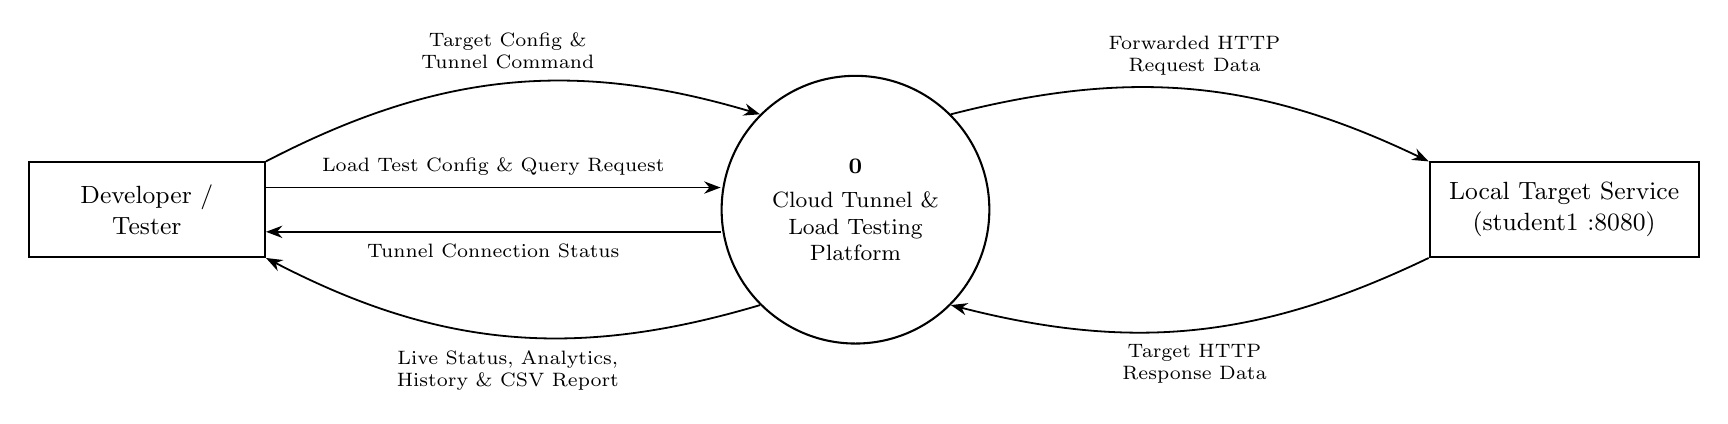
\begin{tikzpicture}

  \node[dfd entity] (user)   at (0, 0) {Developer /\\Tester};
  \node[dfd proc, minimum size=3.4cm] (sys) at (9.0, 0) {\textbf{0}\\[3pt]Cloud Tunnel \&\\Load Testing\\Platform};
  \node[dfd entity] (target) at (18.0, 0) {Local Target Service\\(student1 :8080)};

  \draw[uml arrow] (user.north east) to[bend left=22] node[lbl, above=3pt] {Target Config \&\\Tunnel Command} (sys.north west);
  \draw[uml arrow] ([yshift=8pt]user.east) -- node[lbl, above=2pt] {Load Test Config \& Query Request} ([yshift=8pt]sys.west);
  \draw[uml arrow] ([yshift=-8pt]sys.west) -- node[lbl, below=2pt] {Tunnel Connection Status} ([yshift=-8pt]user.east);
  \draw[uml arrow] (sys.south west) to[bend left=22] node[lbl, below=3pt] {Live Status, Analytics,\\History \& CSV Report} (user.south east);

  \draw[uml arrow] (sys.north east) to[bend left=20] node[lbl, above=3pt] {Forwarded HTTP\\Request Data} (target.north west);
  \draw[uml arrow] (target.south west) to[bend left=20] node[lbl, below=3pt] {Target HTTP\\Response Data} (sys.south east);

\end{tikzpicture}%
}
\caption{DFD Level 0 (Context Diagram): Single System Process and External Entities (No Data Stores).}
\label{fig:dfd0}
\end{figure}

\subsection{DFD Level 1}

Figure~\ref{fig:dfd1} decomposes Process \texttt{0} into five core processes (\texttt{1.0}--\texttt{5.0}) and three persistent stores (\texttt{D1}--\texttt{D3}), preserving all six external flows from Level 0.

\begin{figure}[!htbp]
\centering
\resizebox{\linewidth}{!}{%
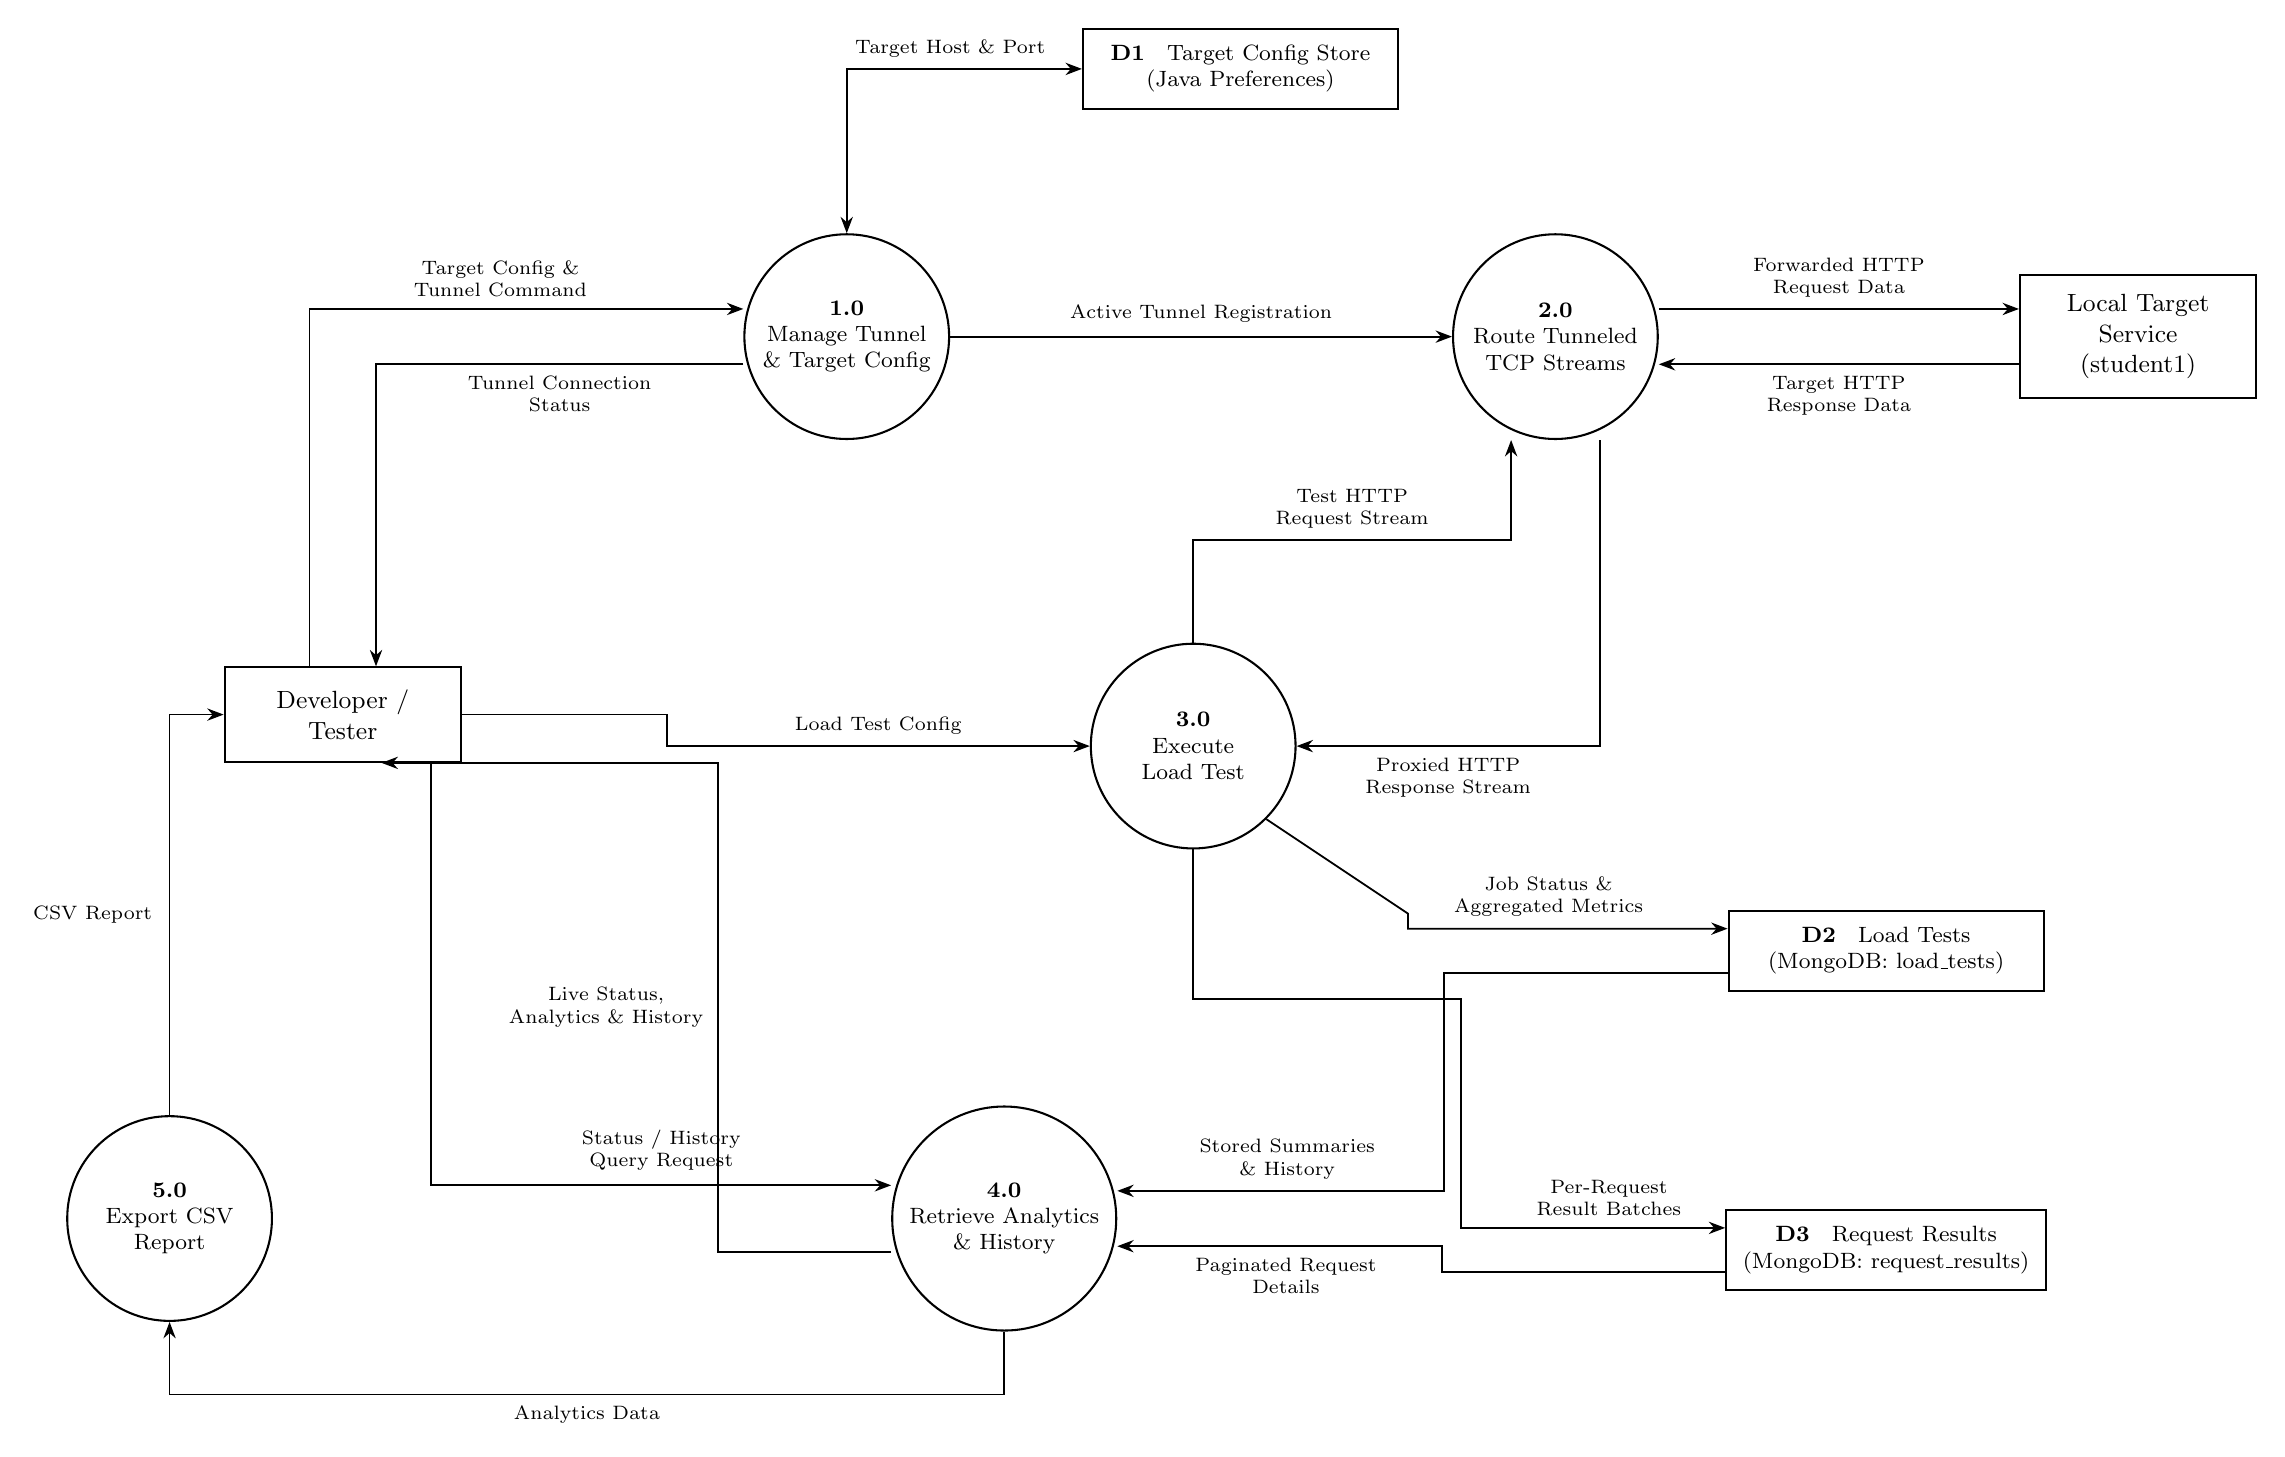
\begin{tikzpicture}

  % Generously spaced coordinates (width ~24cm, height ~16cm, scaled cleanly)
  \node[dfd entity] (user)   at (0, -5.8)  {Developer /\\Tester};
  \node[dfd entity] (target) at (22.8, -1.0) {Local Target\\Service\\(student1)};

  \node[dfd proc] (p1) at (6.4,  -1.0)  {\textbf{1.0}\\Manage Tunnel\\\& Target Config};
  \node[dfd proc] (p2) at (15.4, -1.0)  {\textbf{2.0}\\Route Tunneled\\TCP Streams};
  \node[dfd proc] (p3) at (10.8, -6.2)  {\textbf{3.0}\\Execute\\Load Test};
  \node[dfd proc] (p4) at (8.4,  -12.2) {\textbf{4.0}\\Retrieve Analytics\\\& History};
  \node[dfd proc] (p5) at (-2.2, -12.2) {\textbf{5.0}\\Export CSV\\Report};

  \node[dfd store] (d1) at (11.4,  2.4)  {\textbf{D1} \; Target Config Store\\(Java Preferences)};
  \node[dfd store] (d2) at (19.6, -8.8)  {\textbf{D2} \; Load Tests\\(MongoDB: load\_tests)};
  \node[dfd store] (d3) at (19.6, -12.6) {\textbf{D3} \; Request Results\\(MongoDB: request\_results)};

  % User <-> 1.0
  \draw[uml arrow] ([xshift=-12pt]user.north) |- node[lbl, pos=0.72, above=2pt] {Target Config \&\\Tunnel Command} ([yshift=10pt]p1.west);
  \draw[uml arrow] ([yshift=-10pt]p1.west) -| node[lbl, pos=0.25, below=2pt] {Tunnel Connection\\Status} ([xshift=12pt]user.north);

  % 1.0 <-> D1
  \draw[uml biarrow] (p1.north) |- node[lbl, pos=0.72, above=2pt] {Target Host \& Port} (d1.west);

  % 1.0 -> 2.0
  \draw[uml arrow] (p1.east) -- node[lbl, above=3pt] {Active Tunnel Registration} (p2.west);

  % 2.0 <-> Target
  \draw[uml arrow] ([yshift=10pt]p2.east) -- node[lbl, above=2pt] {Forwarded HTTP\\Request Data} ([yshift=10pt]target.west);
  \draw[uml arrow] ([yshift=-10pt]target.west) -- node[lbl, below=2pt] {Target HTTP\\Response Data} ([yshift=-10pt]p2.east);

  % User -> 3.0
  \draw[uml arrow] (user.east) -- ++(2.6, 0) |- node[lbl, pos=0.75, above=2pt] {Load Test Config} (p3.west);

  % 3.0 <-> 2.0
  \draw[uml arrow] (p3.north) -- ++(0, 1.3) -| node[lbl, pos=0.25, above=2pt] {Test HTTP\\Request Stream} ([xshift=-16pt]p2.south);
  \draw[uml arrow] ([xshift=16pt]p2.south) |- node[lbl, pos=0.75, below=2pt] {Proxied HTTP\\Response Stream} (p3.east);

  % 3.0 -> D2 & D3
  \draw[uml arrow] (p3.south east) -- ++(1.8, -1.2) |- node[lbl, pos=0.72, above=2pt] {Job Status \&\\Aggregated Metrics} ([yshift=8pt]d2.west);
  \draw[uml arrow] (p3.south) -- ++(0, -1.9) -| ++(3.4, -2.5) |- node[lbl, pos=0.78, above=2pt] {Per-Request\\Result Batches} ([yshift=8pt]d3.west);

  % D2 & D3 -> 4.0
  \draw[uml arrow] ([yshift=-8pt]d2.west) -- ++(-3.6, 0) |- node[lbl, pos=0.74, above=2pt] {Stored Summaries\\\& History} ([yshift=10pt]p4.east);
  \draw[uml arrow] ([yshift=-8pt]d3.west) -| ++(-3.6, 0) |- node[lbl, pos=0.74, below=2pt] {Paginated Request\\Details} ([yshift=-10pt]p4.east);

  % User <-> 4.0 (routed cleanly right of 5.0, ZERO crossing!)
  \draw[uml arrow] ([xshift=32pt]user.south) |- node[lbl, pos=0.75, above=3pt] {Status / History\\Query Request} ([yshift=12pt]p4.west);
  \draw[uml arrow] ([yshift=-12pt]p4.west) -- ++(-2.2, 0) |- node[lbl, pos=0.25, left=3pt] {Live Status,\\Analytics \& History} ([xshift=14pt]user.south);

  % 4.0 -> 5.0 -> User (5.0 sits directly below User!)
  \draw[uml arrow] (p4.south) -- ++(0, -0.8) -| node[lbl, pos=0.25, below=2pt] {Analytics Data} (p5.south);
  \draw[uml arrow] (p5.north) |- node[lbl, pos=0.25, left=4pt] {CSV Report} (user.west);

\end{tikzpicture}%
}
\caption{DFD Level 1: Balanced Decomposition into Five Core Processes and Three Data Stores.}
\label{fig:dfd1}
\end{figure}

\subsection{DFD Level 2}

Figures~\ref{fig:dfd2a} and~\ref{fig:dfd2b} explode Process \texttt{2.0} (\textit{Route Tunneled TCP Streams}) and Process \texttt{3.0} (\textit{Execute Load Test}) into balanced sub-processes.

\begin{figure}[!htbp]
\centering
\resizebox{\linewidth}{!}{%
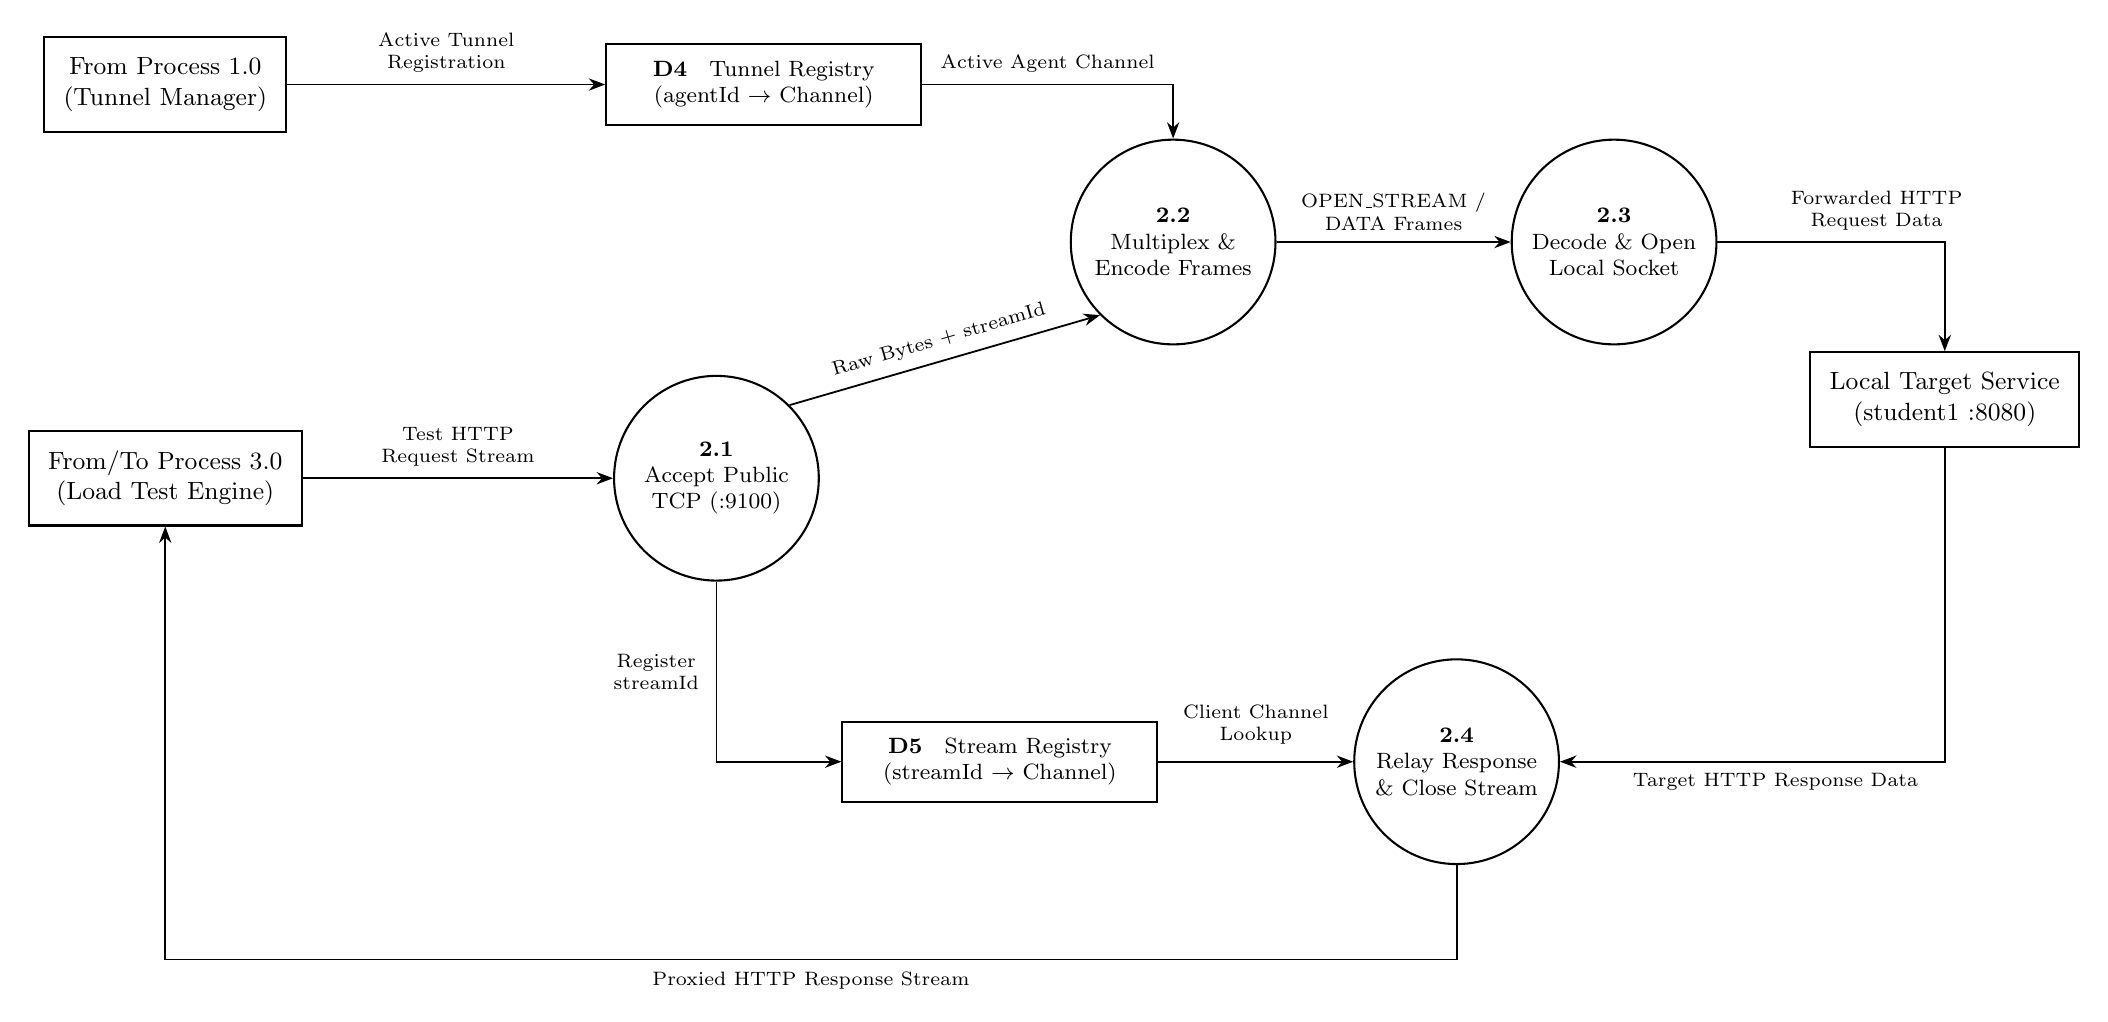
\begin{tikzpicture}

  % Wide 4-column layout with ZERO crossing lines
  \node[dfd entity] (from1)  at (0,    4.0) {From Process 1.0\\(Tunnel Manager)};
  \node[dfd entity] (from3)  at (0,   -1.0) {From/To Process 3.0\\(Load Test Engine)};
  \node[dfd entity] (target) at (22.6, 0.0) {Local Target Service\\(student1 :8080)};

  \node[dfd store] (d4) at (7.6,  4.0) {\textbf{D4} \; Tunnel Registry\\(agentId $\to$ Channel)};
  \node[dfd store] (d5) at (10.6, -4.6) {\textbf{D5} \; Stream Registry\\(streamId $\to$ Channel)};

  \node[dfd proc] (p21) at (7.0,  -1.0) {\textbf{2.1}\\Accept Public\\TCP (:9100)};
  \node[dfd proc] (p22) at (12.8,  2.0) {\textbf{2.2}\\Multiplex \&\\Encode Frames};
  \node[dfd proc] (p23) at (18.4,  2.0) {\textbf{2.3}\\Decode \& Open\\Local Socket};
  \node[dfd proc] (p24) at (16.4, -4.6) {\textbf{2.4}\\Relay Response\\\& Close Stream};

  \draw[uml arrow] (from1.east) -- node[lbl, above=2pt] {Active Tunnel\\Registration} (d4.west);
  \draw[uml arrow] (d4.east) -| node[lbl, pos=0.25, above=2pt] {Active Agent Channel} (p22.north);
  \draw[uml arrow] (from3.east) -- node[lbl, above=2pt] {Test HTTP\\Request Stream} (p21.west);
  \draw[uml arrow] (p21.south) |- node[lbl, pos=0.25, left=4pt] {Register\\streamId} (d5.west);
  \draw[uml arrow] (p21.north east) -- node[lbl, sloped, above=2pt] {Raw Bytes + streamId} (p22.south west);
  \draw[uml arrow] (p22.east) -- node[lbl, above=2pt] {OPEN\_STREAM /\\DATA Frames} (p23.west);
  \draw[uml arrow] (p23.east) -| node[lbl, pos=0.35, above=2pt] {Forwarded HTTP\\Request Data} (target.north);
  \draw[uml arrow] (target.south) |- node[lbl, pos=0.72, below=2pt] {Target HTTP Response Data} (p24.east);
  \draw[uml arrow] (d5.east) -- node[lbl, above=4pt] {Client Channel\\Lookup} (p24.west);

  % Return to Process 3.0 routed cleanly BELOW D5 (zero crossing!)
  \draw[uml arrow] (p24.south) -- ++(0, -1.2) -| node[lbl, pos=0.25, below=2pt] {Proxied HTTP Response Stream} (from3.south);

\end{tikzpicture}%
}
\caption{DFD Level 2 (Case A): Explosion of Process 2.0 (Route Tunneled TCP Streams).}
\label{fig:dfd2a}
\end{figure}

\begin{figure}[!htbp]
\centering
\resizebox{\linewidth}{!}{%
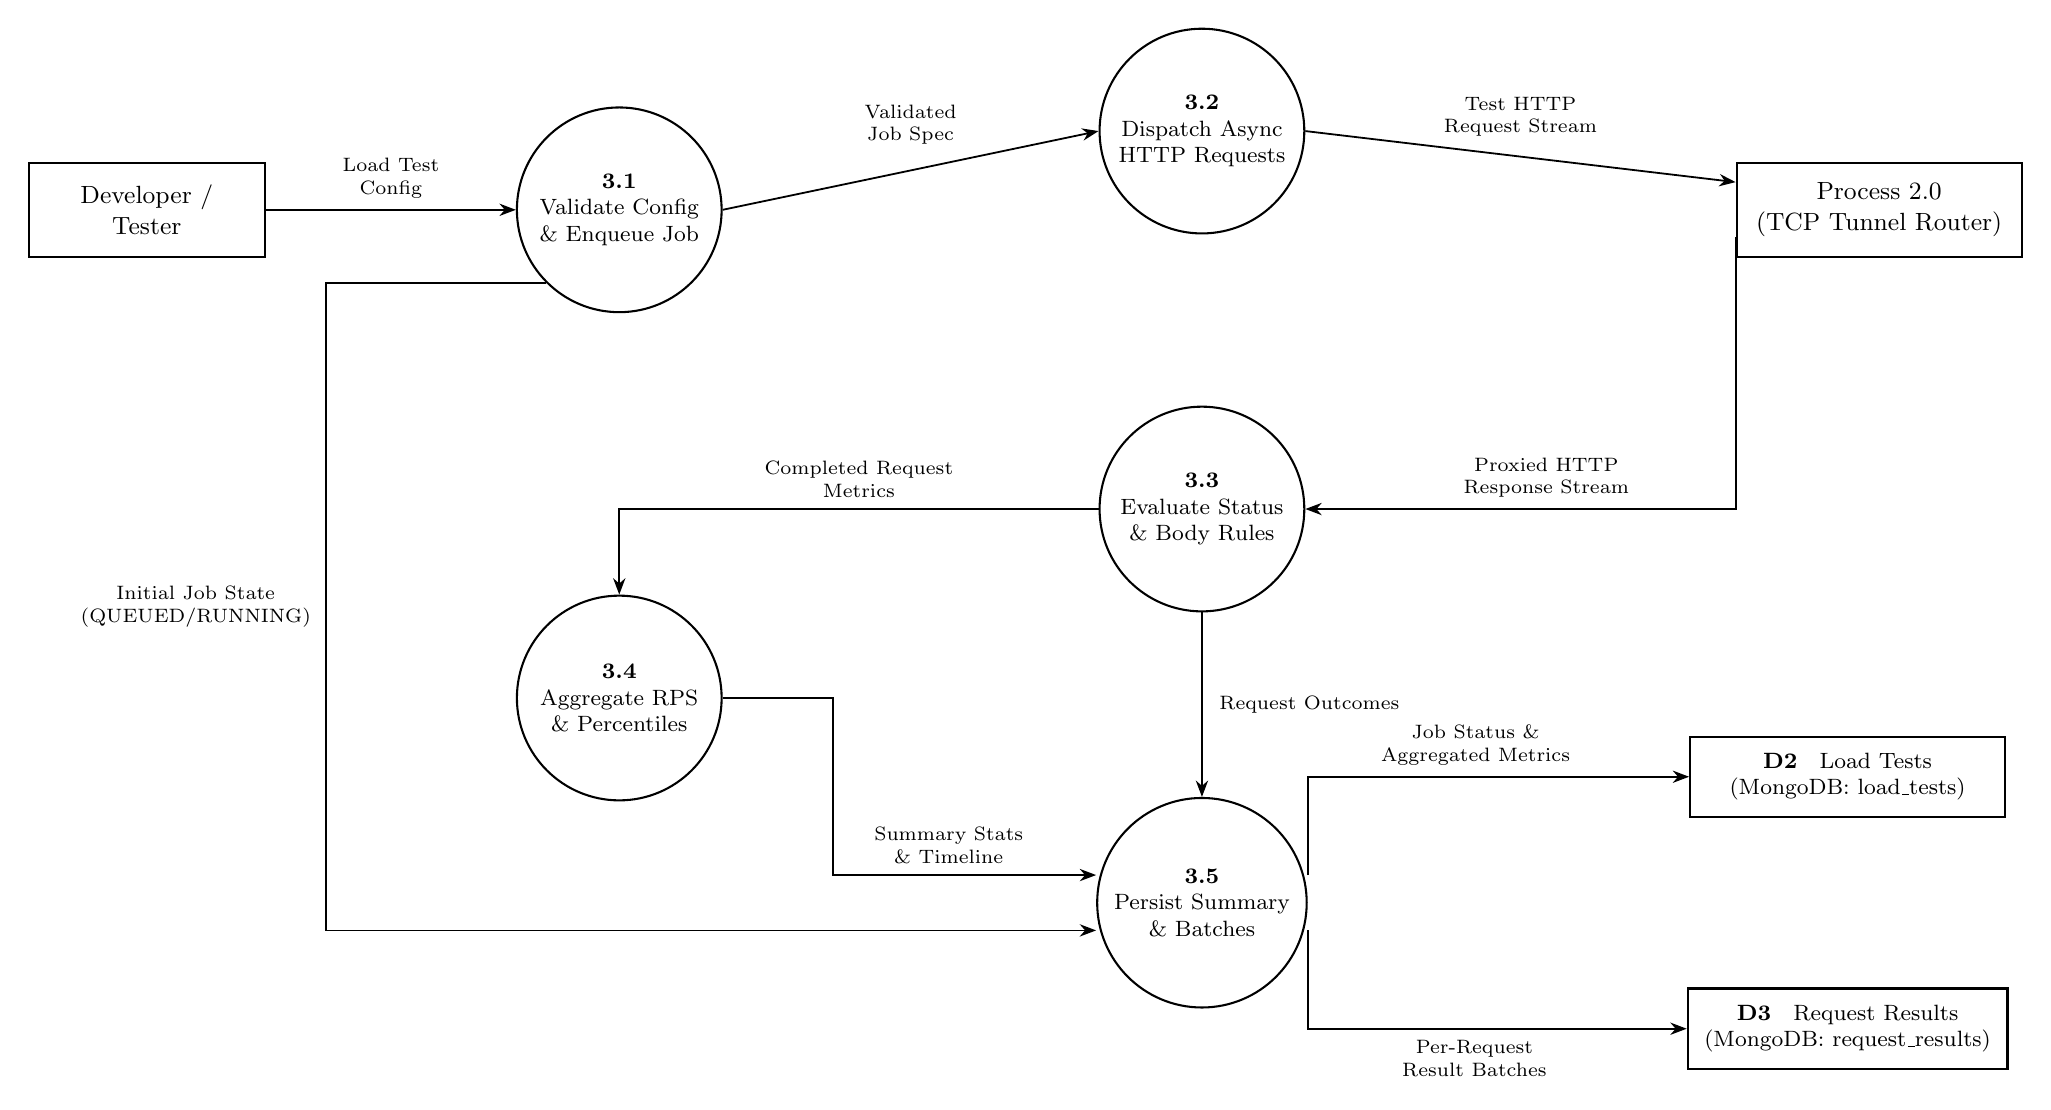
\begin{tikzpicture}

  \node[dfd entity] (user) at (0,    2.6) {Developer /\\Tester};
  \node[dfd entity] (p2)   at (22.0, 2.6) {Process 2.0\\(TCP Tunnel Router)};

  \node[dfd proc] (p31) at (6.0,   2.6) {\textbf{3.1}\\Validate Config\\\& Enqueue Job};
  \node[dfd proc] (p32) at (13.4,  3.6) {\textbf{3.2}\\Dispatch Async\\HTTP Requests};
  \node[dfd proc] (p33) at (13.4, -1.2) {\textbf{3.3}\\Evaluate Status\\\& Body Rules};
  \node[dfd proc] (p34) at (6.0,  -3.6) {\textbf{3.4}\\Aggregate RPS\\\& Percentiles};
  \node[dfd proc] (p35) at (13.4, -6.2) {\textbf{3.5}\\Persist Summary\\\& Batches};

  \node[dfd store] (d2) at (21.6, -4.6) {\textbf{D2} \; Load Tests\\(MongoDB: load\_tests)};
  \node[dfd store] (d3) at (21.6, -7.8) {\textbf{D3} \; Request Results\\(MongoDB: request\_results)};

  \draw[uml arrow] (user.east) -- node[lbl, above=2pt] {Load Test\\Config} (p31.west);
  \draw[uml arrow] (p31.east) -- node[lbl, above=7pt] {Validated\\Job Spec} (p32.west);

  % Initial Job State routed cleanly via left outer margin around 3.4 (ZERO crossing!)
  \draw[uml arrow] (p31.south west) -- ++(-2.8, 0) |- node[lbl, pos=0.25, left=3pt] {Initial Job State\\(QUEUED/RUNNING)} ([yshift=-10pt]p35.west);

  \draw[uml arrow] (p32.east) -- node[lbl, above=5pt] {Test HTTP\\Request Stream} ([yshift=10pt]p2.west);
  \draw[uml arrow] ([yshift=-10pt]p2.west) |- node[lbl, pos=0.72, above=2pt] {Proxied HTTP\\Response Stream} (p33.east);
  \draw[uml arrow] (p33.west) -| node[lbl, pos=0.25, above=2pt] {Completed Request\\Metrics} (p34.north);
  \draw[uml arrow] (p33.south) -- node[lbl, right=4pt] {Request Outcomes} (p35.north);
  \draw[uml arrow] (p34.east) -- ++(1.4, 0) |- node[lbl, pos=0.72, above=2pt] {Summary Stats\\\& Timeline} ([yshift=10pt]p35.west);
  \draw[uml arrow] ([yshift=10pt]p35.east) |- node[lbl, pos=0.72, above=2pt] {Job Status \&\\Aggregated Metrics} (d2.west);
  \draw[uml arrow] ([yshift=-10pt]p35.east) |- node[lbl, pos=0.72, below=2pt] {Per-Request\\Result Batches} (d3.west);

\end{tikzpicture}%
}
\caption{DFD Level 2 (Case B): Explosion of Process 3.0 (Execute Load Test).}
\label{fig:dfd2b}
\end{figure}

\section{Software Requirement Specification in IEEE Format}

\textbf{1. Introduction:} This IEEE-style SRS defines requirements for the \textit{Cloud Tunnel Gateway and Local Load Testing Platform} (V1), comprising \texttt{LocalLoadAgent}, \texttt{CloudTunnelGateway} on AWS EC2, and the \texttt{student1} target service.\\
\textbf{2. Overall Description:} Designed for developers and QA testers. Operating environment: Java 21 + JavaFX 21.0.6 + Netty 4.1.118 + Jackson 2.18.2 on the local workstation; Java 17 + Spring Boot 4.1.1 + Netty 4.1.118 + MongoDB (\texttt{:27017}) on AWS EC2; Java 17 Spring Boot JDBC (\texttt{student1}) + MySQL Test Database (\texttt{:3306}) locally. System limits: 100,000 requests/test, concurrency 1,000, timeout 60,000\,ms, 1\,MB payload cap, 4 worker threads, 20 queued jobs.\\
\textbf{3. Functional Requirements:}
\begin{itemize}
  \item \textbf{FR-1 (Target Config):} Persist host/port via \texttt{TargetConfigurationStore} (Java \texttt{Preferences}).
  \item \textbf{FR-2 (Tunneling):} Maintain outbound Netty tunnel to AWS EC2 (\texttt{:9090}) with \texttt{REGISTER}/\texttt{REGISTER\_ACK} and live \texttt{ConnectionStatus}.
  \item \textbf{FR-3 (Multiplexing):} Accept TCP on \texttt{:9100}, map \texttt{streamId} in \texttt{StreamRegistry}, and relay \texttt{OPEN\_STREAM}, \texttt{DATA}, and \texttt{CLOSE\_STREAM} frames.
  \item \textbf{FR-4 (Submission):} Validate and enqueue async jobs via \texttt{POST /api/load-tests} (\texttt{:8081}).
  \item \textbf{FR-5 (Assertions):} Validate HTTP status, optional body substring, and latency limit; classify failures via \texttt{FailureType}.
  \item \textbf{FR-6 (Analytics \& Storage):} Aggregate RPS, min/max/avg/P50/P95/P99, latency buckets, and timelines; save to \texttt{load\_tests} and batched \texttt{request\_results}.
  \item \textbf{FR-7 (UI Visualisation):} Poll status, render Pie, Throughput, Latency, and Scatter charts plus paginated request details.
  \item \textbf{FR-8 (History \& Export):} Paginate MongoDB test history and export full results to CSV.
\end{itemize}
\textbf{4. Non-Functional Requirements:} Non-blocking Netty I/O and async \texttt{HttpClient} (verified at 664.41 attempts/sec over 10,000 requests); bounded buffers (100 pending chunks/stream, 20 queued jobs); clean dark-themed JavaFX UI; modular three-project Maven separation.

\section{User Stories and Story Cards}

\begin{table}[!htbp]
\centering
\small
\caption{Product Backlog User Stories}
\label{tab:userstories}
\begin{tabularx}{\linewidth}{|L{1.2cm}|Y|L{1.6cm}|}
\hline
\textbf{ID} & \textbf{User Story} & \textbf{Priority} \\
\hline
US-01 & As a developer, I want to configure my local target port and connect a reverse tunnel to the AWS EC2 gateway so that my \texttt{localhost} service can be load-tested securely. & High \\
\hline
US-02 & As a developer, I want to configure HTTP method, headers, query parameters, body, total requests, concurrency, and timeout to simulate realistic traffic. & High \\
\hline
US-03 & As a tester, I want to define expected HTTP status codes and response-body assertions so that functional regressions under load are flagged automatically. & High \\
\hline
US-04 & As a tester, I want to monitor live test progress and view throughput, outcome pie, latency distribution, and per-request scatter charts to pinpoint bottlenecks. & High \\
\hline
US-05 & As a developer, I want to inspect paginated per-request latencies and error classifications to distinguish timeouts from HTTP status failures. & Medium \\
\hline
US-06 & As a developer, I want to browse historical load test runs persisted in MongoDB to compare performance across builds. & Medium \\
\hline
US-07 & As a tester, I want to export summary KPIs, throughput timelines, and request rows to CSV for offline analysis. & Medium \\
\hline
\end{tabularx}
\end{table}

\textbf{Example Story Card --- US-04 (Monitor Live Execution and View Analytics):} Submitting a valid test opens \texttt{TestExecutionView} and polls \texttt{GET /api/load-tests/\{testId\}} until \texttt{COMPLETED}/\texttt{FAILED}; KPI cards display Total, Passed, Failed, Errors, RPS, Avg, Min, Max, P50, P95, and P99; all four charts populate automatically; clicking any scatter dot inspects its exact status and latency.

% =====================================================================
% CHAPTER 3: DESIGN PHASE
% =====================================================================
\chapter{Design Phase}

Each design diagram below models two significant cases directly grounded in the implemented classes and runtime workflows.

\section{Class Diagram}

Figures~\ref{fig:class1} and~\ref{fig:class2} detail the Netty tunnel multiplexing classes and the asynchronous load-testing and MongoDB persistence classes.

\begin{figure}[!htbp]
\centering
\resizebox{\linewidth}{!}{%
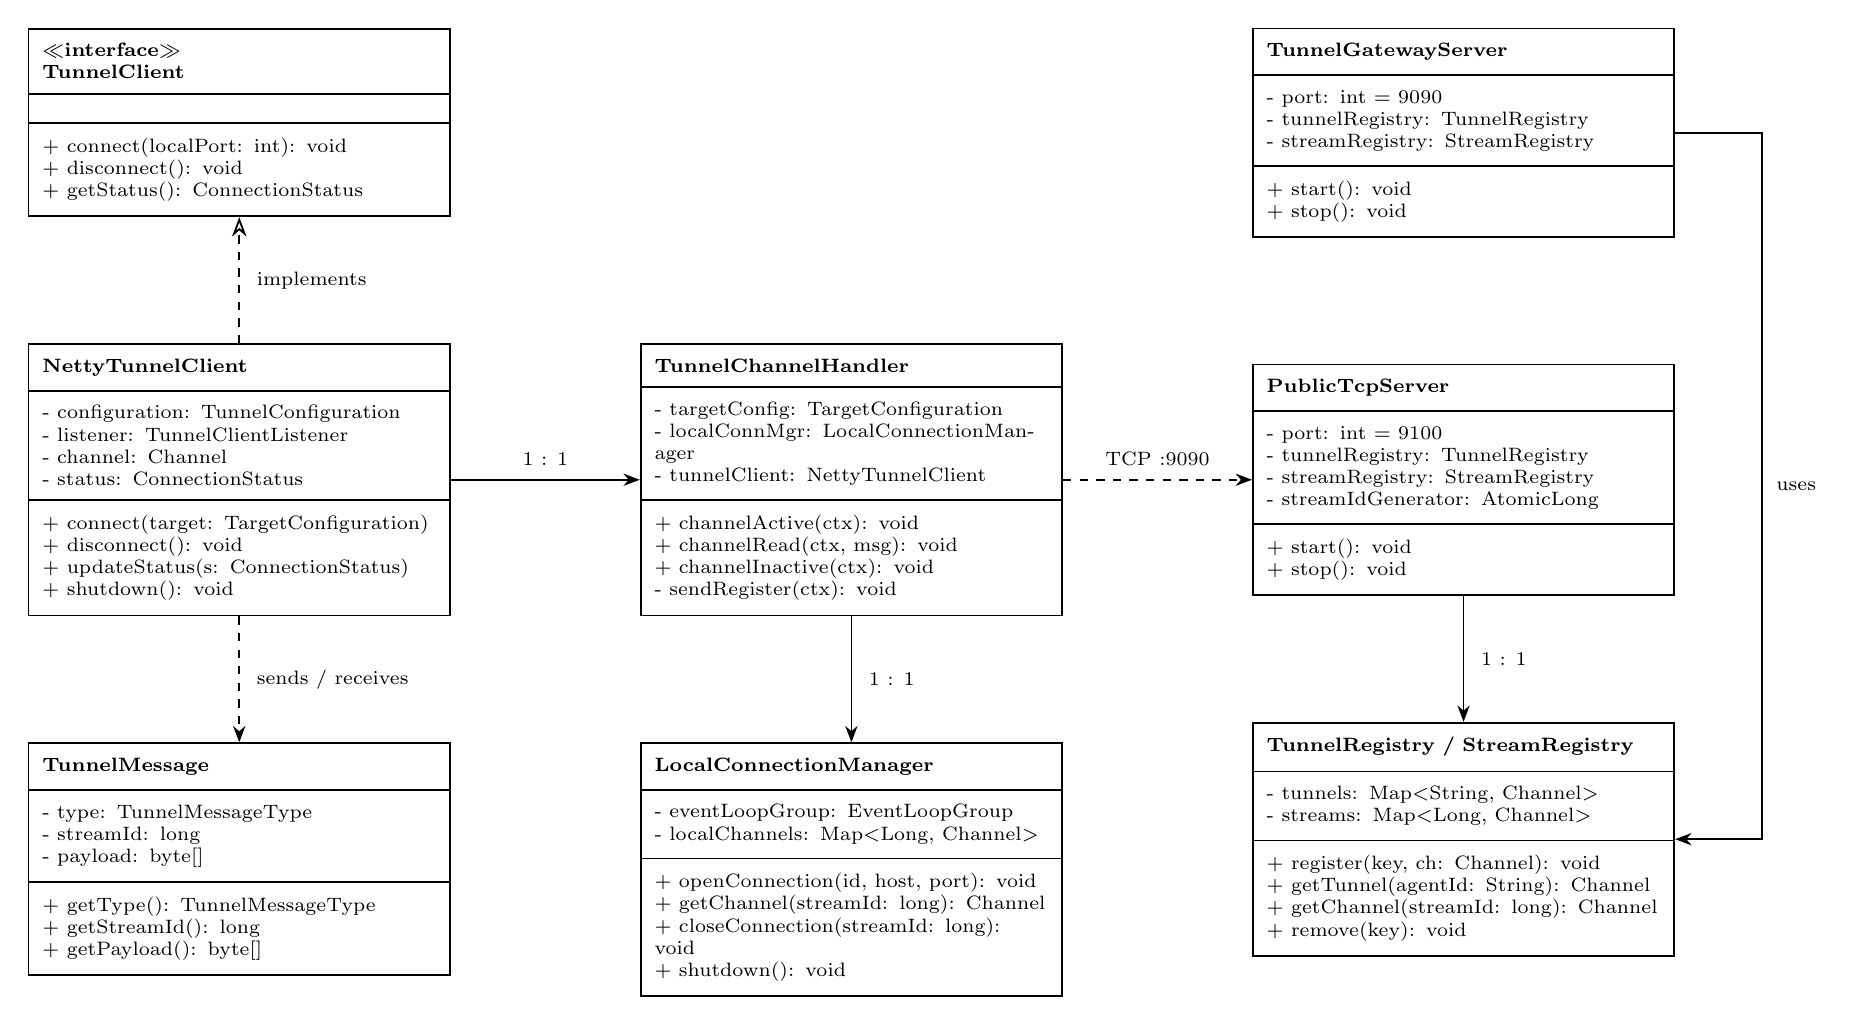
\begin{tikzpicture}[node distance=1.8cm and 2.4cm]

  % Left column (relative vertical positioning -> mathematically IMPOSSIBLE to overlap!)
  \node[uml class, text width=5.0cm] (tc) {
    \textbf{$\ll$interface$\gg$}\\
    \textbf{TunnelClient}
    \nodepart{two}
    \nodepart{three}
    + connect(localPort: int): void\\
    + disconnect(): void\\
    + getStatus(): ConnectionStatus
  };

  \node[uml class, text width=5.0cm, below=1.6cm of tc] (ntc) {
    \textbf{NettyTunnelClient}
    \nodepart{two}
    - configuration: TunnelConfiguration\\
    - listener: TunnelClientListener\\
    - channel: Channel\\
    - status: ConnectionStatus
    \nodepart{three}
    + connect(target: TargetConfiguration)\\
    + disconnect(): void\\
    + updateStatus(s: ConnectionStatus)\\
    + shutdown(): void
  };

  \node[uml class, text width=5.0cm, below=1.6cm of ntc] (msg) {
    \textbf{TunnelMessage}
    \nodepart{two}
    - type: TunnelMessageType\\
    - streamId: long\\
    - payload: byte[]
    \nodepart{three}
    + getType(): TunnelMessageType\\
    + getStreamId(): long\\
    + getPayload(): byte[]
  };

  % Middle column
  \node[uml class, text width=5.0cm, right=2.4cm of ntc] (tch) {
    \textbf{TunnelChannelHandler}
    \nodepart{two}
    - targetConfig: TargetConfiguration\\
    - localConnMgr: LocalConnectionManager\\
    - tunnelClient: NettyTunnelClient
    \nodepart{three}
    + channelActive(ctx): void\\
    + channelRead(ctx, msg): void\\
    + channelInactive(ctx): void\\
    - sendRegister(ctx): void
  };

  \node[uml class, text width=5.0cm, below=1.6cm of tch] (lcm) {
    \textbf{LocalConnectionManager}
    \nodepart{two}
    - eventLoopGroup: EventLoopGroup\\
    - localChannels: Map$<$Long, Channel$>$
    \nodepart{three}
    + openConnection(id, host, port): void\\
    + getChannel(streamId: long): Channel\\
    + closeConnection(streamId: long): void\\
    + shutdown(): void
  };

  % Right column (aligned cleanly via positioning)
  \node[uml class, text width=5.0cm, right=2.4cm of tch] (pts) {
    \textbf{PublicTcpServer}
    \nodepart{two}
    - port: int = 9100\\
    - tunnelRegistry: TunnelRegistry\\
    - streamRegistry: StreamRegistry\\
    - streamIdGenerator: AtomicLong
    \nodepart{three}
    + start(): void\\
    + stop(): void
  };

  \node[uml class, text width=5.0cm, above=1.6cm of pts] (tgs) {
    \textbf{TunnelGatewayServer}
    \nodepart{two}
    - port: int = 9090\\
    - tunnelRegistry: TunnelRegistry\\
    - streamRegistry: StreamRegistry
    \nodepart{three}
    + start(): void\\
    + stop(): void
  };

  \node[uml class, text width=5.0cm, below=1.6cm of pts] (reg) {
    \textbf{TunnelRegistry / StreamRegistry}
    \nodepart{two}
    - tunnels: Map$<$String, Channel$>$\\
    - streams: Map$<$Long, Channel$>$
    \nodepart{three}
    + register(key, ch: Channel): void\\
    + getTunnel(agentId: String): Channel\\
    + getChannel(streamId: long): Channel\\
    + remove(key): void
  };

  % Clean connectors inside guaranteed 1.6cm/2.4cm gaps
  \draw[uml dasharrow, -{Stealth[open, length=7pt]}] (ntc.north) -- node[lbl, right=4pt] {implements} (tc.south);
  \draw[uml arrow] (ntc.east) -- node[lbl, above=3pt] {1 : 1} (tch.west);
  \draw[uml arrow] (tch.south) -- node[lbl, right=4pt] {1 : 1} (lcm.north);
  \draw[uml dasharrow] (ntc.south) -- node[lbl, right=4pt] {sends / receives} (msg.north);
  \draw[uml arrow] (tgs.east) -- ++(1.1, 0) |- node[lbl, pos=0.25, right=3pt] {uses} (reg.east);
  \draw[uml arrow] (pts.south) -- node[lbl, right=4pt] {1 : 1} (reg.north);
  \draw[uml dasharrow] (tch.east) -- node[lbl, above=3pt] {TCP :9090} (pts.west);

\end{tikzpicture}%
}
\caption{Class Diagram (Case 1): Netty Tunnel Client, Gateway Server, and Stream Multiplexing Subsystem.}
\label{fig:class1}
\end{figure}

\begin{figure}[!htbp]
\centering
\resizebox{\linewidth}{!}{%
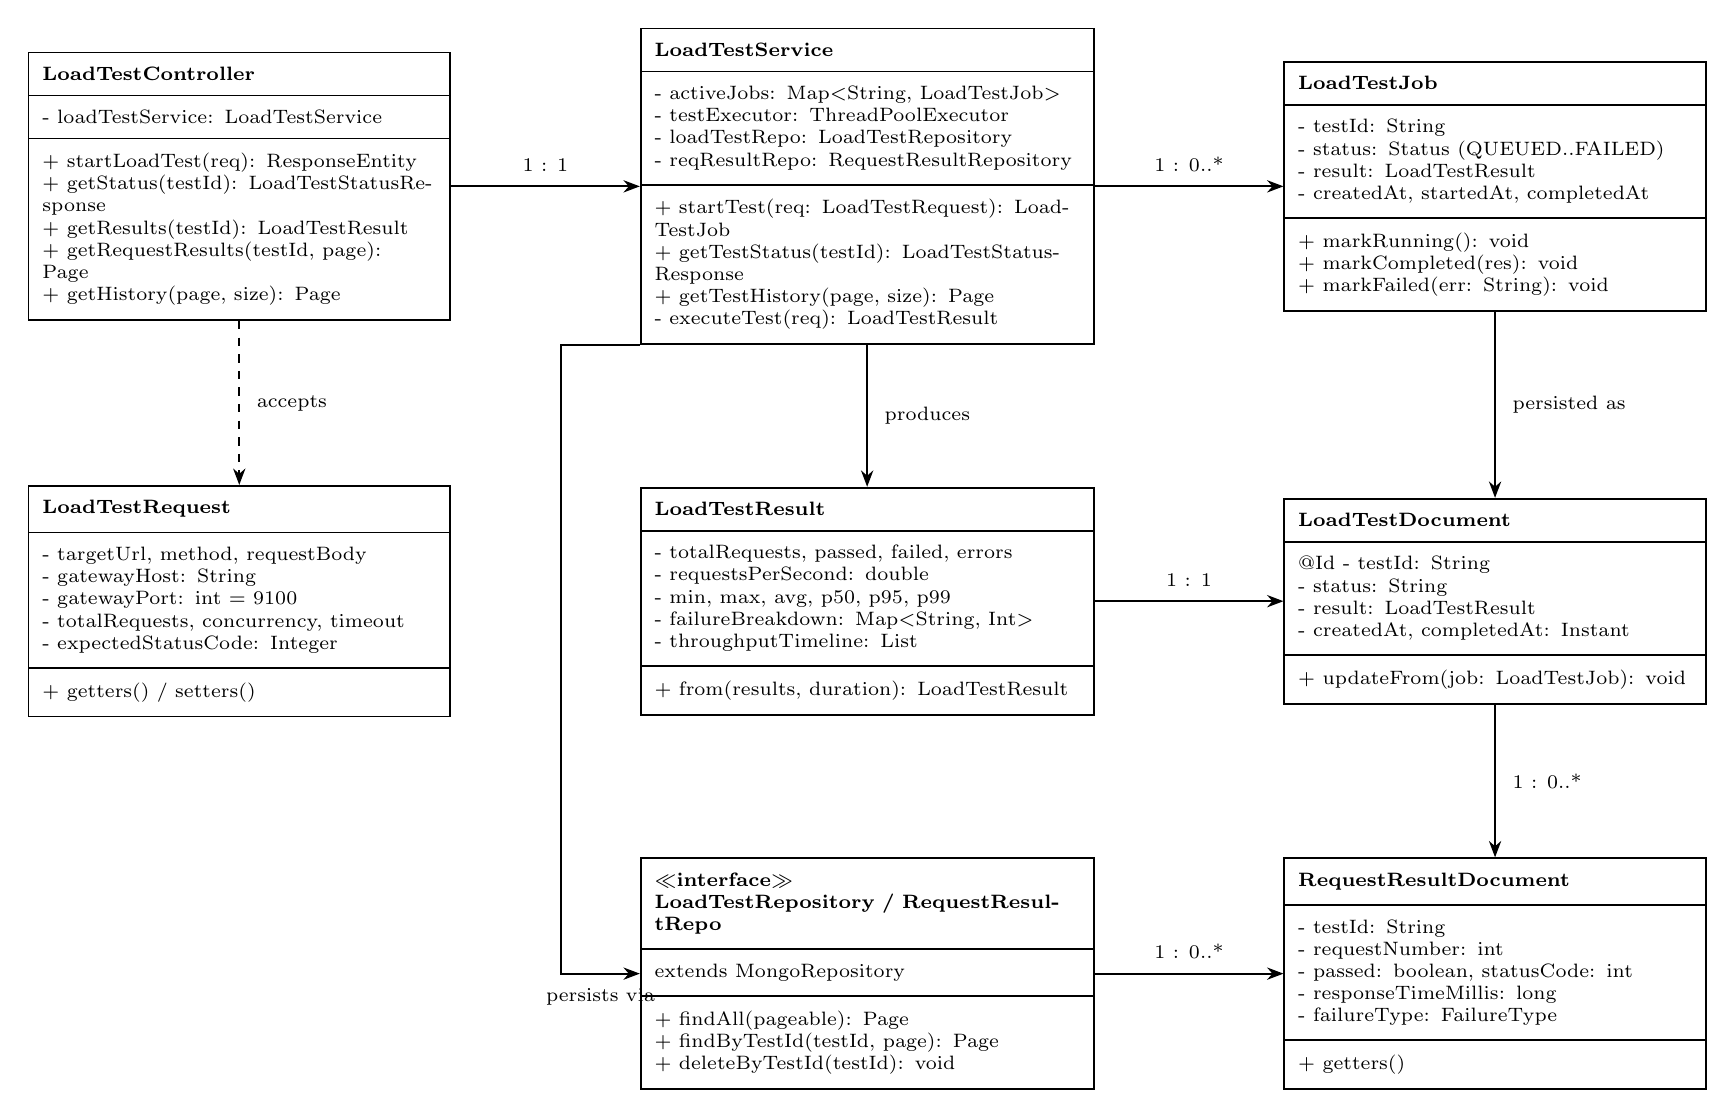
\begin{tikzpicture}[node distance=1.8cm and 2.4cm]

  % Top row (relative positioning -> ZERO overlaps!)
  \node[uml class, text width=5.0cm] (ctrl) {
    \textbf{LoadTestController}
    \nodepart{two}
    - loadTestService: LoadTestService
    \nodepart{three}
    + startLoadTest(req): ResponseEntity\\
    + getStatus(testId): LoadTestStatusResponse\\
    + getResults(testId): LoadTestResult\\
    + getRequestResults(testId, page): Page\\
    + getHistory(page, size): Page
  };

  \node[uml class, text width=5.4cm, right=2.4cm of ctrl] (svc) {
    \textbf{LoadTestService}
    \nodepart{two}
    - activeJobs: Map$<$String, LoadTestJob$>$\\
    - testExecutor: ThreadPoolExecutor\\
    - loadTestRepo: LoadTestRepository\\
    - reqResultRepo: RequestResultRepository
    \nodepart{three}
    + startTest(req: LoadTestRequest): LoadTestJob\\
    + getTestStatus(testId): LoadTestStatusResponse\\
    + getTestHistory(page, size): Page\\
    - executeTest(req): LoadTestResult
  };

  \node[uml class, text width=5.0cm, right=2.4cm of svc] (job) {
    \textbf{LoadTestJob}
    \nodepart{two}
    - testId: String\\
    - status: Status (QUEUED..FAILED)\\
    - result: LoadTestResult\\
    - createdAt, startedAt, completedAt
    \nodepart{three}
    + markRunning(): void\\
    + markCompleted(res): void\\
    + markFailed(err: String): void
  };

  % Middle row (explicitly below tallest box in top row!)
  \node[uml class, text width=5.4cm, below=1.8cm of svc] (res) {
    \textbf{LoadTestResult}
    \nodepart{two}
    - totalRequests, passed, failed, errors\\
    - requestsPerSecond: double\\
    - min, max, avg, p50, p95, p99\\
    - failureBreakdown: Map$<$String, Int$>$\\
    - throughputTimeline: List
    \nodepart{three}
    + from(results, duration): LoadTestResult
  };

  \node[uml class, text width=5.0cm, left=2.4cm of res] (req) {
    \textbf{LoadTestRequest}
    \nodepart{two}
    - targetUrl, method, requestBody\\
    - gatewayHost: String\\
    - gatewayPort: int = 9100\\
    - totalRequests, concurrency, timeout\\
    - expectedStatusCode: Integer
    \nodepart{three}
    + getters() / setters()
  };

  \node[uml class, text width=5.0cm, right=2.4cm of res] (doc) {
    \textbf{LoadTestDocument}
    \nodepart{two}
    @Id - testId: String\\
    - status: String\\
    - result: LoadTestResult\\
    - createdAt, completedAt: Instant
    \nodepart{three}
    + updateFrom(job: LoadTestJob): void
  };

  % Bottom row
  \node[uml class, text width=5.4cm, below=1.8cm of res] (repo) {
    \textbf{$\ll$interface$\gg$}\\
    \textbf{LoadTestRepository / RequestResultRepo}
    \nodepart{two}
    extends MongoRepository
    \nodepart{three}
    + findAll(pageable): Page\\
    + findByTestId(testId, page): Page\\
    + deleteByTestId(testId): void
  };

  \node[uml class, text width=5.0cm, right=2.4cm of repo] (rdoc) {
    \textbf{RequestResultDocument}
    \nodepart{two}
    - testId: String\\
    - requestNumber: int\\
    - passed: boolean, statusCode: int\\
    - responseTimeMillis: long\\
    - failureType: FailureType
    \nodepart{three}
    + getters()
  };

  % Clean connectors inside guaranteed wide gaps
  \draw[uml arrow] (ctrl.east) -- node[lbl, above=3pt] {1 : 1} (svc.west);
  \draw[uml arrow] (svc.east) -- node[lbl, above=3pt] {1 : 0..*} (job.west);
  \draw[uml dasharrow] (ctrl.south) -- node[lbl, right=4pt] {accepts} (req.north);
  \draw[uml arrow] (svc.south) -- node[lbl, right=4pt] {produces} (res.north);
  \draw[uml arrow] (job.south) -- node[lbl, right=4pt] {persisted as} (doc.north);
  \draw[uml arrow] (res.east) -- node[lbl, above=3pt] {1 : 1} (doc.west);
  \draw[uml arrow] (svc.south west) -- ++(-1.0, 0) |- node[lbl, pos=0.75, below=3pt] {persists via} (repo.west);
  \draw[uml arrow] (repo.east) -- node[lbl, above=3pt] {1 : 0..*} (rdoc.west);
  \draw[uml arrow] (doc.south) -- node[lbl, right=4pt] {1 : 0..*} (rdoc.north);

\end{tikzpicture}%
}
\caption{Class Diagram (Case 2): Load Testing, Analytics Aggregation, and MongoDB Persistence Subsystem.}
\label{fig:class2}
\end{figure}

\section{Sequence Diagrams}

\subsection{Tunnel Registration and Proxied Request Relay}
Figure~\ref{fig:seq1} traces \texttt{NettyTunnelClient} registration with \texttt{TunnelGatewayServer} on AWS EC2 (\texttt{:9090}) and proxied forwarding from \texttt{PublicTcpServer} (\texttt{:9100}) to \texttt{student1} (\texttt{:8080}).

\begin{figure}[!htbp]
\centering
\resizebox{\linewidth}{!}{%
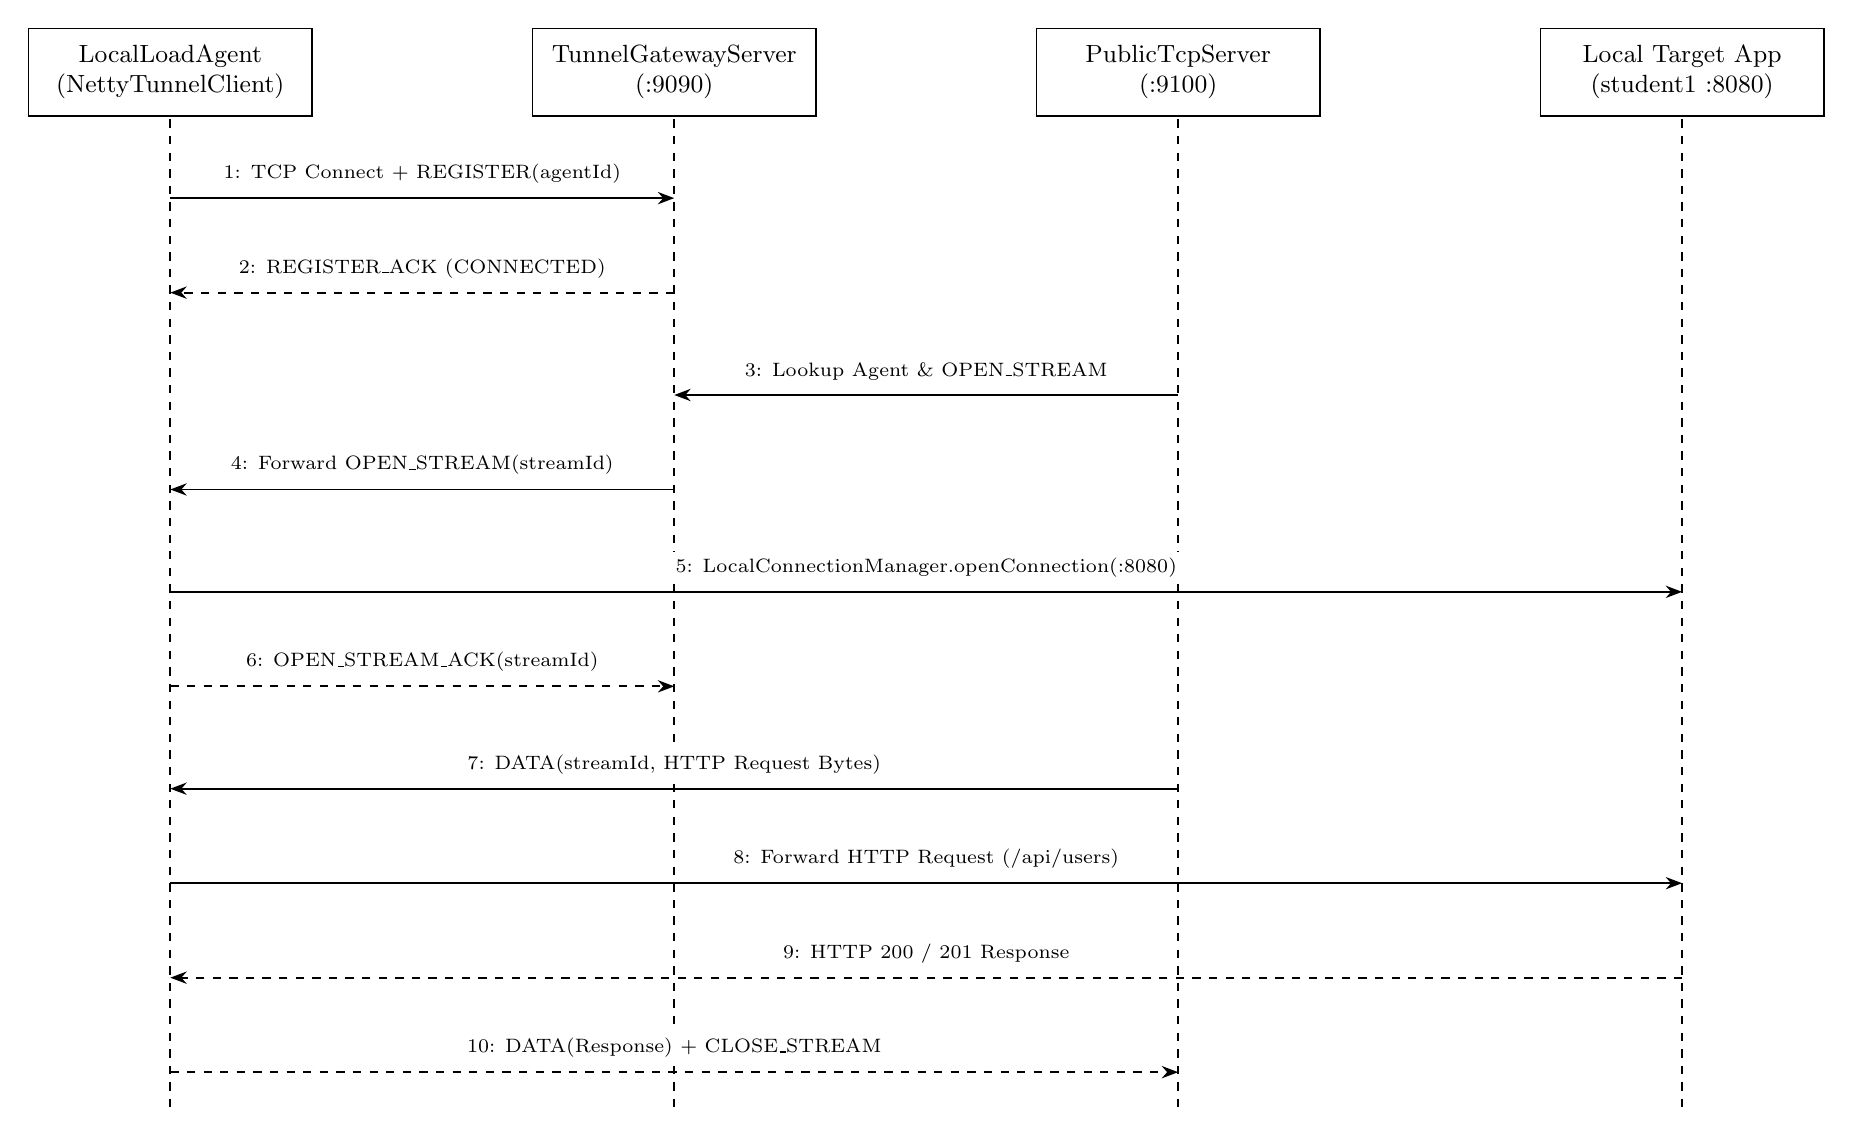
\begin{tikzpicture}

  % Lifelines spaced 6.4cm apart so NO label ever crosses a dashed lifeline!
  \node[uml box, minimum width=3.6cm] (l1) at (0,    0) {LocalLoadAgent\\(NettyTunnelClient)};
  \node[uml box, minimum width=3.6cm] (l2) at (6.4,  0) {TunnelGatewayServer\\(:9090)};
  \node[uml box, minimum width=3.6cm] (l3) at (12.8, 0) {PublicTcpServer\\(:9100)};
  \node[uml box, minimum width=3.6cm] (l4) at (19.2, 0) {Local Target App\\(student1 :8080)};

  \foreach \x in {0, 6.4, 12.8, 19.2}{
    \draw[dashed, black, line width=0.6pt] (\x, -0.6) -- (\x, -13.2);
  }

  \draw[uml arrow]     (0,    -1.6) -- node[lbl, fill=white, above=3pt] {1: TCP Connect + REGISTER(agentId)} (6.4,  -1.6);
  \draw[uml dasharrow] (6.4,  -2.8) -- node[lbl, fill=white, above=3pt] {2: REGISTER\_ACK (CONNECTED)} (0,    -2.8);

  \draw[uml arrow]     (12.8, -4.1) -- node[lbl, fill=white, above=3pt] {3: Lookup Agent \& OPEN\_STREAM} (6.4,  -4.1);
  \draw[uml arrow]     (6.4,  -5.3) -- node[lbl, fill=white, above=3pt] {4: Forward OPEN\_STREAM(streamId)} (0,    -5.3);
  \draw[uml arrow]     (0,    -6.6) -- node[lbl, fill=white, above=3pt] {5: LocalConnectionManager.openConnection(:8080)} (19.2, -6.6);
  \draw[uml dasharrow] (0,    -7.8) -- node[lbl, fill=white, above=3pt] {6: OPEN\_STREAM\_ACK(streamId)} (6.4,  -7.8);

  \draw[uml arrow]     (12.8, -9.1) -- node[lbl, fill=white, above=3pt] {7: DATA(streamId, HTTP Request Bytes)} (0,    -9.1);
  \draw[uml arrow]     (0,   -10.3) -- node[lbl, fill=white, above=3pt] {8: Forward HTTP Request (/api/users)} (19.2, -10.3);
  \draw[uml dasharrow] (19.2,-11.5) -- node[lbl, fill=white, above=3pt] {9: HTTP 200 / 201 Response} (0,   -11.5);
  \draw[uml dasharrow] (0,   -12.7) -- node[lbl, fill=white, above=3pt] {10: DATA(Response) + CLOSE\_STREAM} (12.8,-12.7);

\end{tikzpicture}%
}
\caption{Sequence Diagram (Case 1): Tunnel Registration and Proxied TCP/HTTP Stream Relay.}
\label{fig:seq1}
\end{figure}

\subsection{Asynchronous Load Test Execution and Polling}
Figure~\ref{fig:seq2} traces REST submission (\texttt{POST /api/load-tests}), MongoDB persistence, status polling, and analytics retrieval.

\begin{figure}[!htbp]
\centering
\resizebox{\linewidth}{!}{%
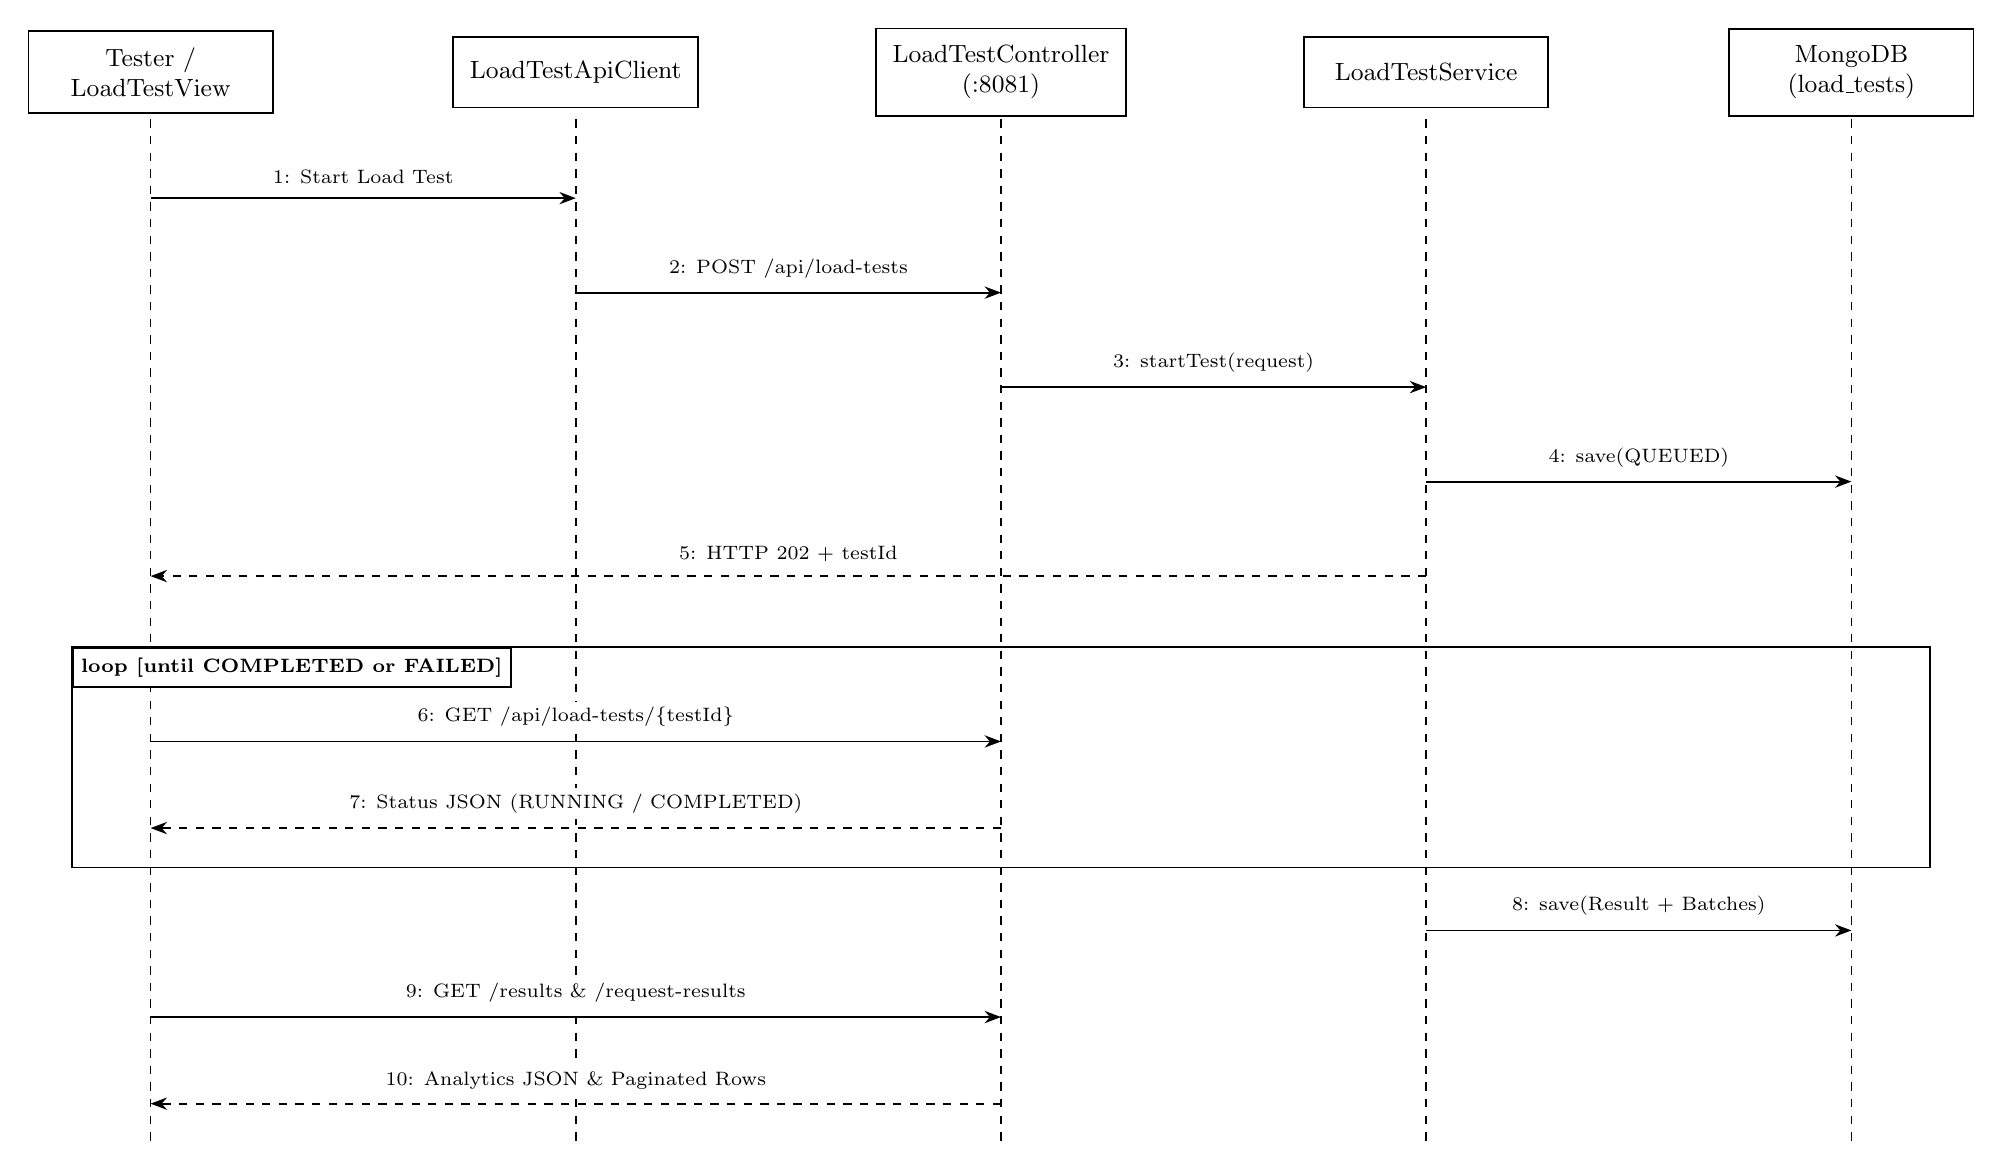
\begin{tikzpicture}

  % Lifelines spaced 5.4cm apart so every label fits cleanly inside its column!
  \node[uml box, minimum width=3.1cm] (s1) at (0,    0) {Tester /\\LoadTestView};
  \node[uml box, minimum width=3.1cm] (s2) at (5.4,  0) {LoadTestApiClient};
  \node[uml box, minimum width=3.1cm] (s3) at (10.8, 0) {LoadTestController\\(:8081)};
  \node[uml box, minimum width=3.1cm] (s4) at (16.2, 0) {LoadTestService};
  \node[uml box, minimum width=3.1cm] (s5) at (21.6, 0) {MongoDB\\(load\_tests)};

  \foreach \x in {0, 5.4, 10.8, 16.2, 21.6}{
    \draw[dashed, black, line width=0.6pt] (\x, -0.6) -- (\x, -13.6);
  }

  \draw[uml arrow]     (0,    -1.6) -- node[lbl, fill=white, above=3pt] {1: Start Load Test} (5.4,  -1.6);
  \draw[uml arrow]     (5.4,  -2.8) -- node[lbl, fill=white, above=3pt] {2: POST /api/load-tests} (10.8, -2.8);
  \draw[uml arrow]     (10.8, -4.0) -- node[lbl, fill=white, above=3pt] {3: startTest(request)} (16.2, -4.0);
  \draw[uml arrow]     (16.2, -5.2) -- node[lbl, fill=white, above=3pt] {4: save(QUEUED)} (21.6, -5.2);
  \draw[uml dasharrow] (16.2, -6.4) -- node[lbl, fill=white, above=3pt] {5: HTTP 202 + testId} (0,    -6.4);

  % Loop frame for status polling
  \draw[black, line width=0.65pt] (-1.0, -7.3) rectangle (22.6, -10.1);
  \node[uml box, font=\scriptsize\bfseries, inner sep=3pt, minimum height=0.5cm, anchor=north west] at (-1.0, -7.3) {loop [until COMPLETED or FAILED]};
  \draw[uml arrow]     (0,    -8.5) -- node[lbl, fill=white, above=3pt] {6: GET /api/load-tests/\{testId\}} (10.8, -8.5);
  \draw[uml dasharrow] (10.8, -9.6) -- node[lbl, fill=white, above=3pt] {7: Status JSON (RUNNING / COMPLETED)} (0,    -9.6);

  \draw[uml arrow]     (16.2,-10.9) -- node[lbl, fill=white, above=3pt] {8: save(Result + Batches)} (21.6,-10.9);
  \draw[uml arrow]     (0,   -12.0) -- node[lbl, fill=white, above=3pt] {9: GET /results \& /request-results} (10.8,-12.0);
  \draw[uml dasharrow] (10.8,-13.1) -- node[lbl, fill=white, above=3pt] {10: Analytics JSON \& Paginated Rows} (0,   -13.1);

\end{tikzpicture}%
}
\caption{Sequence Diagram (Case 2): Asynchronous Load Test Submission, Polling, and Analytics Retrieval.}
\label{fig:seq2}
\end{figure}

\section{Collaboration Diagrams}

\subsection{Tunneled Stream Multiplexing Workflow}
Figure~\ref{fig:collab1} shows structural object links and numbered message exchanges during stream multiplexing.

\begin{figure}[!htbp]
\centering
\resizebox{\linewidth}{!}{%
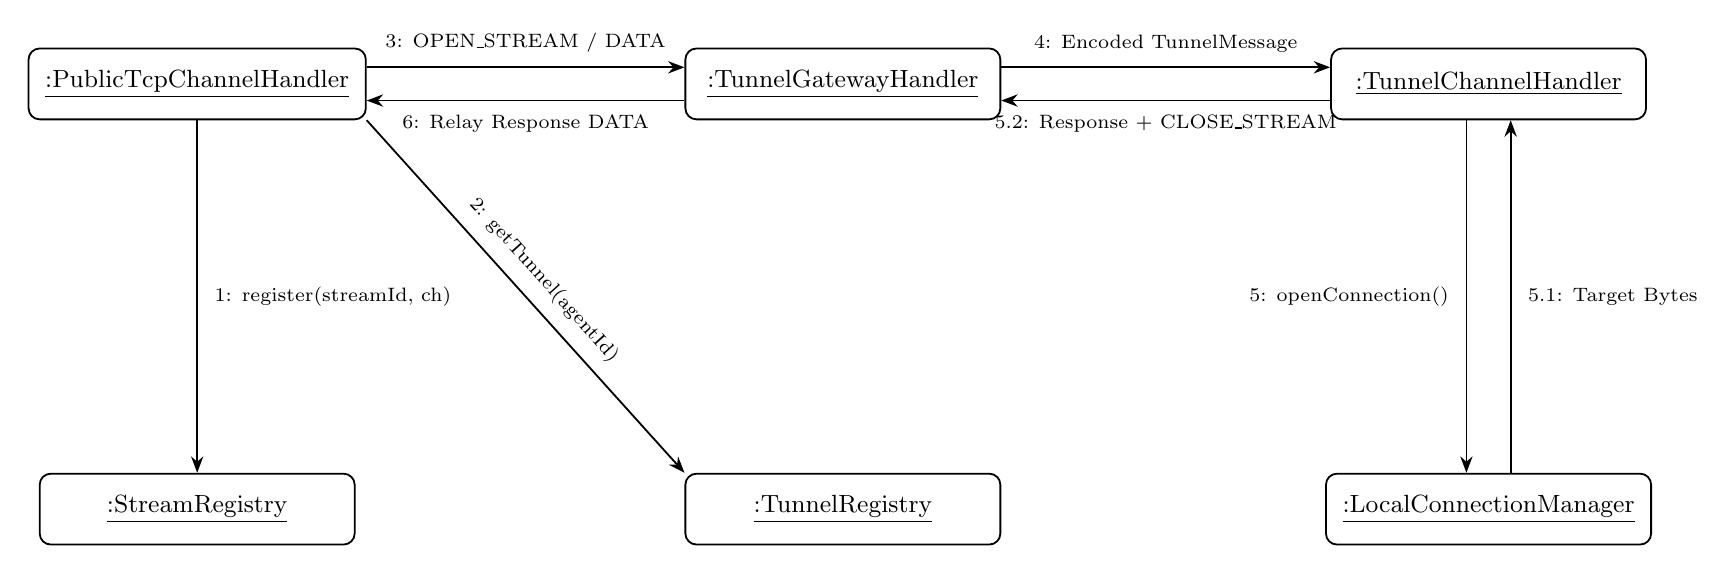
\begin{tikzpicture}

  \node[uml round, minimum width=4.0cm] (c1) at (0,    3.2) {\underline{:PublicTcpChannelHandler}};
  \node[uml round, minimum width=4.0cm] (c2) at (8.2,  3.2) {\underline{:TunnelGatewayHandler}};
  \node[uml round, minimum width=4.0cm] (c3) at (16.4, 3.2) {\underline{:TunnelChannelHandler}};
  \node[uml round, minimum width=4.0cm] (c4) at (16.4,-2.2) {\underline{:LocalConnectionManager}};
  \node[uml round, minimum width=4.0cm] (c5) at (0,   -2.2) {\underline{:StreamRegistry}};
  \node[uml round, minimum width=4.0cm] (c6) at (8.2, -2.2) {\underline{:TunnelRegistry}};

  \draw[uml arrow] (c1.south) -- node[lbl, right=4pt] {1: register(streamId, ch)} (c5.north);
  \draw[uml arrow] (c1.south east) -- node[lbl, sloped, above=3pt] {2: getTunnel(agentId)} (c6.north west);

  \draw[uml arrow] ([yshift=6pt]c1.east)  -- node[lbl, above=3pt] {3: OPEN\_STREAM / DATA} ([yshift=6pt]c2.west);
  \draw[uml arrow] ([yshift=-6pt]c2.west) -- node[lbl, below=3pt] {6: Relay Response DATA} ([yshift=-6pt]c1.east);

  \draw[uml arrow] ([yshift=6pt]c2.east)  -- node[lbl, above=3pt] {4: Encoded TunnelMessage} ([yshift=6pt]c3.west);
  \draw[uml arrow] ([yshift=-6pt]c3.west) -- node[lbl, below=3pt] {5.2: Response + CLOSE\_STREAM} ([yshift=-6pt]c2.east);

  \draw[uml arrow] ([xshift=-8pt]c3.south) -- node[lbl, left=4pt] {5: openConnection()} ([xshift=-8pt]c4.north);
  \draw[uml arrow] ([xshift=8pt]c4.north)  -- node[lbl, right=4pt] {5.1: Target Bytes} ([xshift=8pt]c3.south);

\end{tikzpicture}%
}
\caption{Collaboration Diagram (Case 1): Tunneled Stream Multiplexing and Local Forwarding.}
\label{fig:collab1}
\end{figure}

\subsection{Load Test Execution and Persistence Workflow}
Figure~\ref{fig:collab2} illustrates object collaboration from \texttt{LoadTestView} through \texttt{LoadTestController} and \texttt{LoadTestService} to \texttt{LoadTestRepository}.

\begin{figure}[!htbp]
\centering
\resizebox{\linewidth}{!}{%
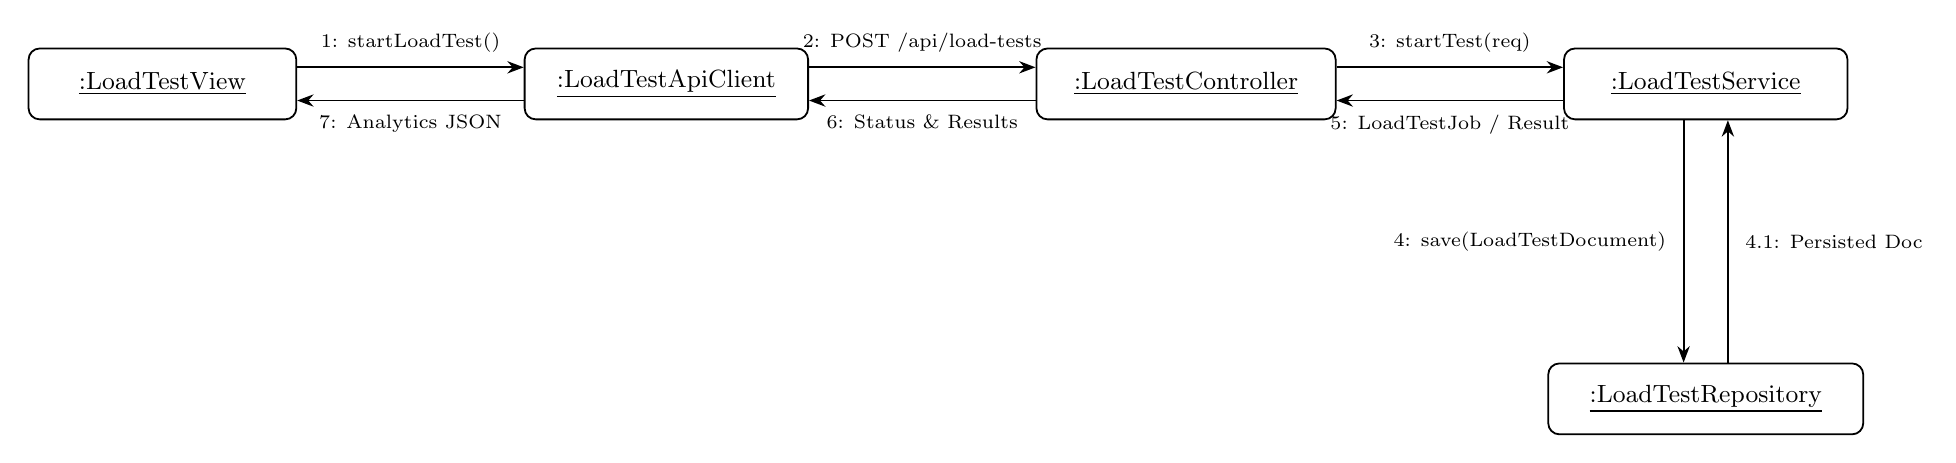
\begin{tikzpicture}

  \node[uml round, minimum width=3.4cm] (m1) at (0,    0) {\underline{:LoadTestView}};
  \node[uml round, minimum width=3.6cm] (m2) at (6.4,  0) {\underline{:LoadTestApiClient}};
  \node[uml round, minimum width=3.8cm] (m3) at (13.0, 0) {\underline{:LoadTestController}};
  \node[uml round, minimum width=3.6cm] (m4) at (19.6, 0) {\underline{:LoadTestService}};
  \node[uml round, minimum width=4.0cm] (m5) at (19.6,-4.0) {\underline{:LoadTestRepository}};

  \draw[uml arrow] ([yshift=6pt]m1.east)  -- node[lbl, above=3pt] {1: startLoadTest()} ([yshift=6pt]m2.west);
  \draw[uml arrow] ([yshift=-6pt]m2.west) -- node[lbl, below=3pt] {7: Analytics JSON} ([yshift=-6pt]m1.east);

  \draw[uml arrow] ([yshift=6pt]m2.east)  -- node[lbl, above=3pt] {2: POST /api/load-tests} ([yshift=6pt]m3.west);
  \draw[uml arrow] ([yshift=-6pt]m3.west) -- node[lbl, below=3pt] {6: Status \& Results} ([yshift=-6pt]m2.east);

  \draw[uml arrow] ([yshift=6pt]m3.east)  -- node[lbl, above=3pt] {3: startTest(req)} ([yshift=6pt]m4.west);
  \draw[uml arrow] ([yshift=-6pt]m4.west) -- node[lbl, below=3pt] {5: LoadTestJob / Result} ([yshift=-6pt]m3.east);

  \draw[uml arrow] ([xshift=-8pt]m4.south) -- node[lbl, left=4pt] {4: save(LoadTestDocument)} ([xshift=-8pt]m5.north);
  \draw[uml arrow] ([xshift=8pt]m5.north)  -- node[lbl, right=4pt] {4.1: Persisted Doc} ([xshift=8pt]m4.south);

\end{tikzpicture}%
}
\caption{Collaboration Diagram (Case 2): Load Test Execution and Persistence Workflow.}
\label{fig:collab2}
\end{figure}

\section{State Chart Diagrams}

\subsection{NettyTunnelClient Connection State}
Figure~\ref{fig:state1} models the five states of \texttt{ConnectionStatus} (\texttt{DISCONNECTED}, \texttt{CONNECTING}, \texttt{CONNECTED}, \texttt{RECONNECTING}, \texttt{ERROR}).

\begin{figure}[!htbp]
\centering
\resizebox{\linewidth}{!}{%
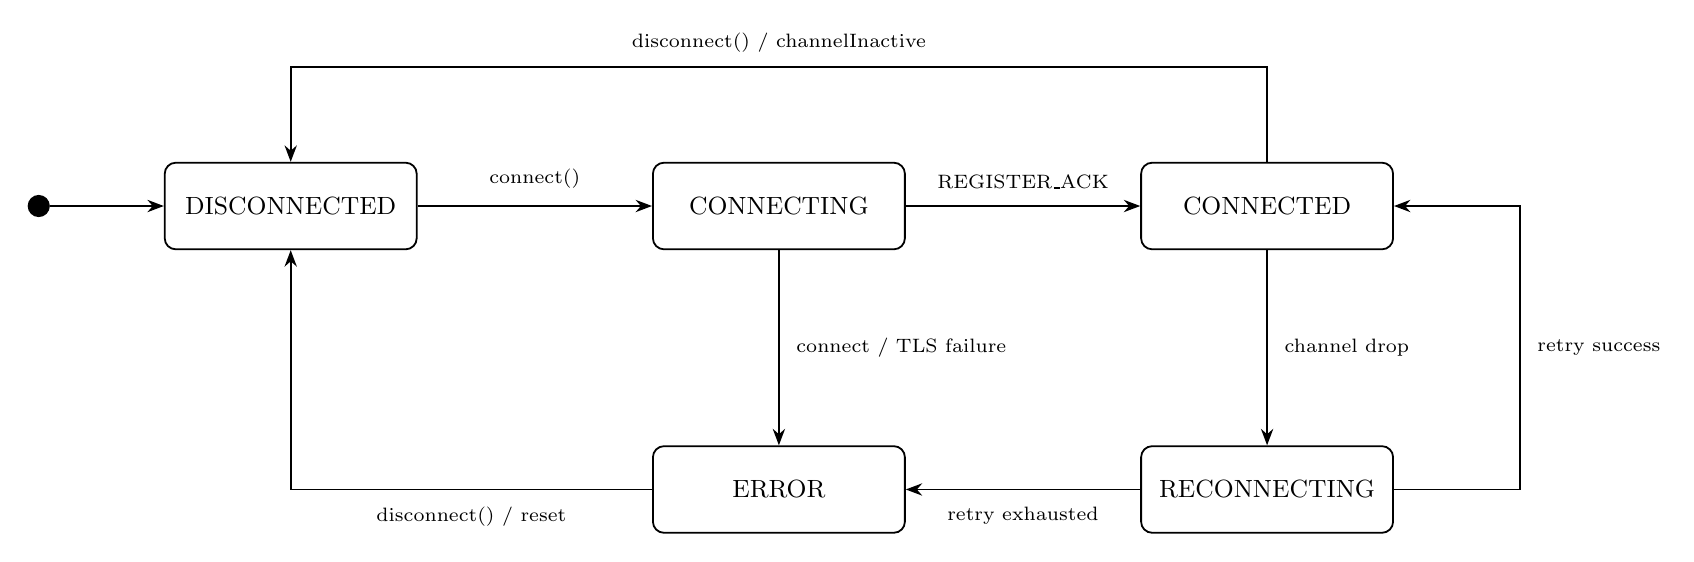
\begin{tikzpicture}

  \node[uml start] (i1) at (-2.4, 0) {};
  \node[uml round, minimum width=3.2cm, minimum height=1.1cm] (st1) at (0.8,  0) {DISCONNECTED};
  \node[uml round, minimum width=3.2cm, minimum height=1.1cm] (st2) at (7.0,  0) {CONNECTING};
  \node[uml round, minimum width=3.2cm, minimum height=1.1cm] (st3) at (13.2, 0) {CONNECTED};
  \node[uml round, minimum width=3.2cm, minimum height=1.1cm] (st4) at (13.2,-3.6) {RECONNECTING};
  \node[uml round, minimum width=3.2cm, minimum height=1.1cm] (st5) at (7.0, -3.6) {ERROR};

  \draw[uml arrow] (i1) -- (st1.west);
  \draw[uml arrow] (st1.east) -- node[lbl, above=4pt] {connect()} (st2.west);
  \draw[uml arrow] (st2.east) -- node[lbl, above=4pt] {REGISTER\_ACK} (st3.west);

  \draw[uml arrow] (st2.south) -- node[lbl, right=4pt] {connect / TLS failure} (st5.north);
  \draw[uml arrow] (st3.south) -- node[lbl, right=4pt] {channel drop} (st4.north);
  \draw[uml arrow] (st4.west) -- node[lbl, below=4pt] {retry exhausted} (st5.east);
  \draw[uml arrow] (st4.east) -- ++(1.6, 0) |- node[lbl, pos=0.25, right=4pt] {retry success} (st3.east);
  \draw[uml arrow] (st3.north) -- ++(0, 1.2) -| node[lbl, pos=0.25, above=3pt] {disconnect() / channelInactive} (st1.north);
  \draw[uml arrow] (st5.west) -| node[lbl, pos=0.25, below=4pt] {disconnect() / reset} (st1.south);

\end{tikzpicture}%
}
\caption{State Chart Diagram (Case 1): NettyTunnelClient Connection Lifecycle (ConnectionStatus).}
\label{fig:state1}
\end{figure}

\subsection{LoadTestJob Execution State}
Figure~\ref{fig:state2} models the four lifecycle states of \texttt{LoadTestJob.Status} (\texttt{QUEUED}, \texttt{RUNNING}, \texttt{COMPLETED}, \texttt{FAILED}).

\begin{figure}[!htbp]
\centering
\resizebox{\linewidth}{!}{%
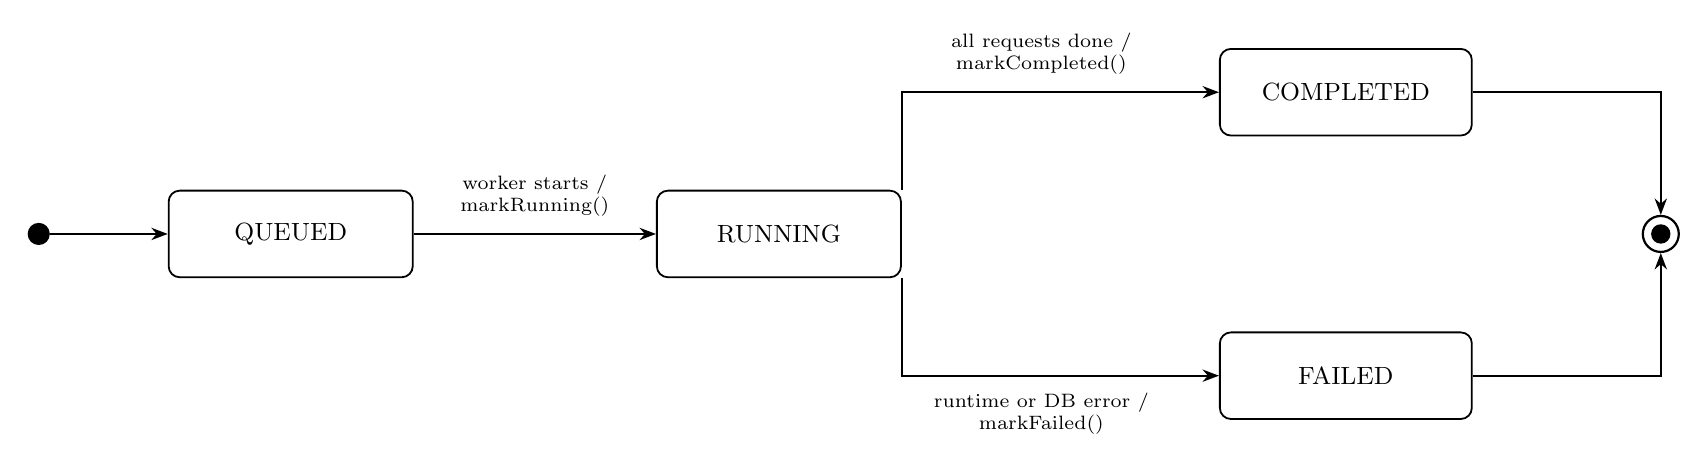
\begin{tikzpicture}

  \node[uml start] (i2) at (-2.4, 0) {};
  \node[uml round, minimum width=3.1cm, minimum height=1.1cm] (j1) at (0.8,  0) {QUEUED};
  \node[uml round, minimum width=3.1cm, minimum height=1.1cm] (j2) at (7.0,  0) {RUNNING};
  \node[uml round, minimum width=3.2cm, minimum height=1.1cm] (j3) at (14.2, 1.8) {COMPLETED};
  \node[uml round, minimum width=3.2cm, minimum height=1.1cm] (j4) at (14.2,-1.8) {FAILED};
  \node[uml end] (f2) at (18.2, 0) {};

  \draw[uml arrow] (i2) -- (j1.west);
  \draw[uml arrow] (j1.east) -- node[lbl, above=4pt] {worker starts /\\markRunning()} (j2.west);
  \draw[uml arrow] (j2.north east) |- node[lbl, pos=0.72, above=4pt] {all requests done /\\markCompleted()} (j3.west);
  \draw[uml arrow] (j2.south east) |- node[lbl, pos=0.72, below=4pt] {runtime or DB error /\\markFailed()} (j4.west);
  \draw[uml arrow] (j3.east) -| (f2.north);
  \draw[uml arrow] (j4.east) -| (f2.south);

\end{tikzpicture}%
}
\caption{State Chart Diagram (Case 2): LoadTestJob Execution Lifecycle (LoadTestJob.Status).}
\label{fig:state2}
\end{figure}

% =====================================================================
% CHAPTER 4: IMPLEMENTATION
% =====================================================================
\chapter{Implementation}

\section{Component Diagrams}

Figure~\ref{fig:comp} presents the component architecture across \texttt{LocalLoadAgent}, \texttt{CloudTunnelGateway} on AWS EC2, MongoDB, and the local \texttt{student1} service backed by the MySQL Test Database.

\begin{figure}[!htbp]
\centering
\resizebox{\linewidth}{!}{%
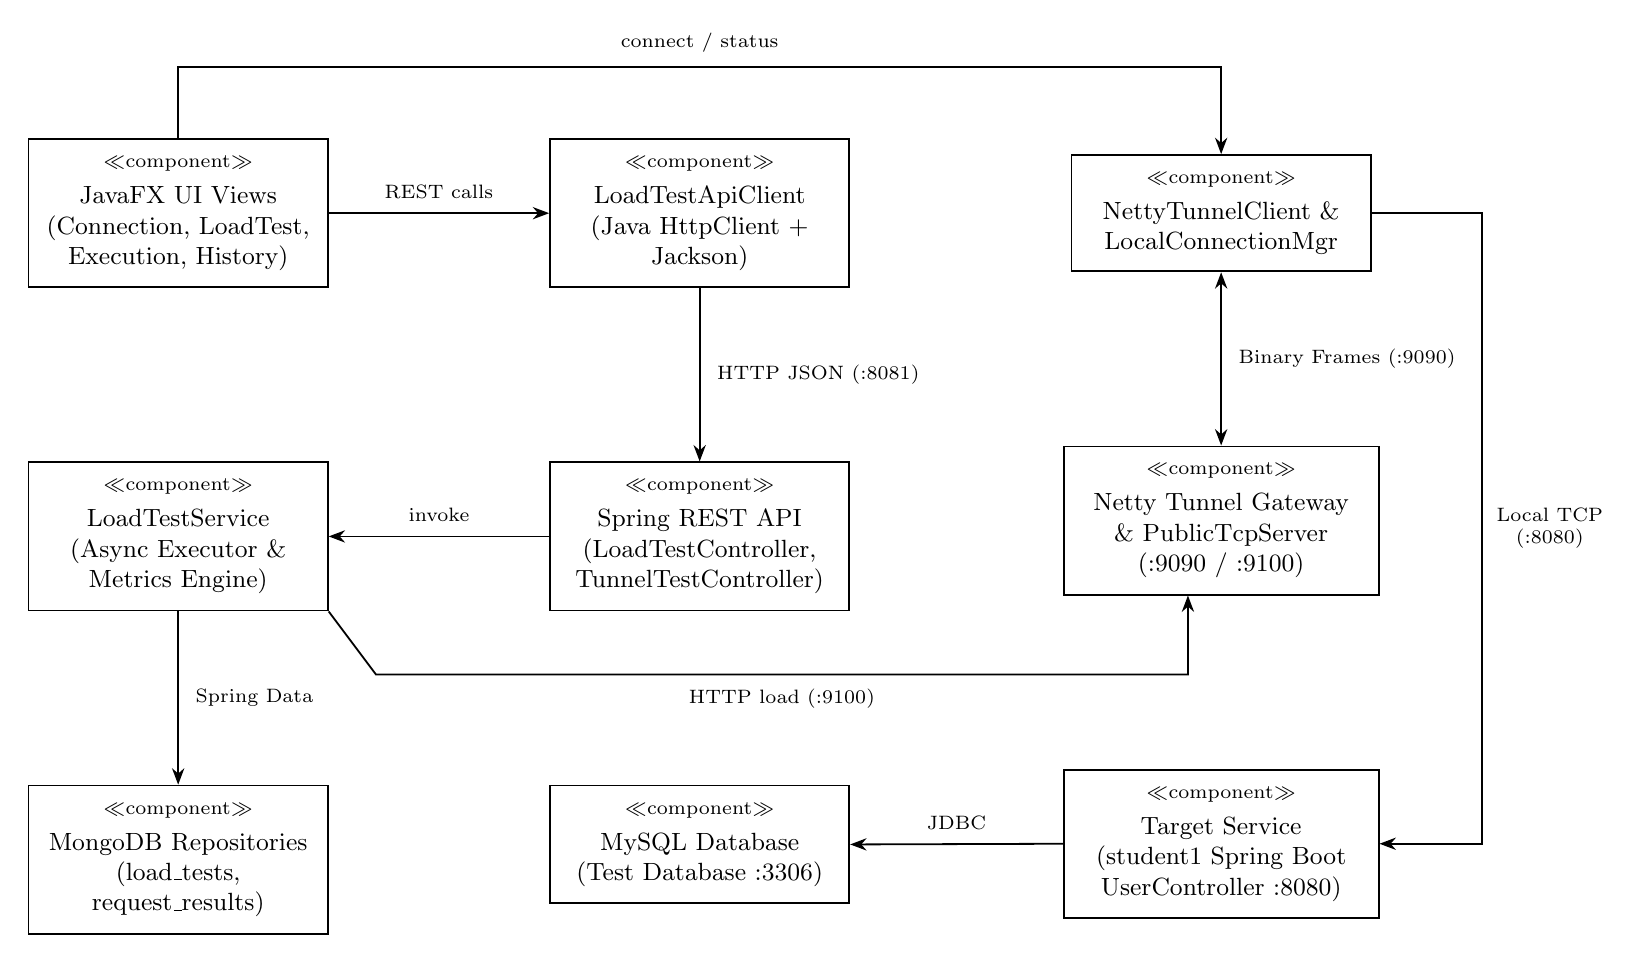
\begin{tikzpicture}[node distance=2.2cm and 2.8cm]

  % Top Row (LocalLoadAgent)
  \node[uml box, minimum width=3.8cm] (ui) {\scriptsize$\ll$component$\gg$\\[2pt]\small JavaFX UI Views\\(Connection, LoadTest,\\Execution, History)};
  \node[uml box, minimum width=3.8cm, right=2.8cm of ui] (api) {\scriptsize$\ll$component$\gg$\\[2pt]\small LoadTestApiClient\\(Java HttpClient +\\Jackson)};
  \node[uml box, minimum width=3.8cm, right=2.8cm of api] (tcli) {\scriptsize$\ll$component$\gg$\\[2pt]\small NettyTunnelClient \&\\LocalConnectionMgr};

  % Middle Row (CloudTunnelGateway)
  \node[uml box, minimum width=3.8cm, below=2.2cm of ui] (lts) {\scriptsize$\ll$component$\gg$\\[2pt]\small LoadTestService\\(Async Executor \&\\Metrics Engine)};
  \node[uml box, minimum width=3.8cm, below=2.2cm of api] (rest) {\scriptsize$\ll$component$\gg$\\[2pt]\small Spring REST API\\(LoadTestController,\\TunnelTestController)};
  \node[uml box, minimum width=4.0cm, below=2.2cm of tcli] (gw) {\scriptsize$\ll$component$\gg$\\[2pt]\small Netty Tunnel Gateway\\\& PublicTcpServer\\(:9090 / :9100)};

  % Bottom Row (Persistence & Target)
  \node[uml box, minimum width=3.8cm, below=2.2cm of lts] (mdb) {\scriptsize$\ll$component$\gg$\\[2pt]\small MongoDB Repositories\\(load\_tests,\\request\_results)};
  \node[uml box, minimum width=3.8cm, below=2.2cm of rest] (mysql) {\scriptsize$\ll$component$\gg$\\[2pt]\small MySQL Database\\(Test Database :3306)};
  \node[uml box, minimum width=4.0cm, below=2.2cm of gw] (st1) {\scriptsize$\ll$component$\gg$\\[2pt]\small Target Service\\(student1 Spring Boot\\UserController :8080)};

  % Clean non-cutting connectors
  \draw[uml arrow] (ui.east) -- node[lbl, above=3pt] {REST calls} (api.west);
  \draw[uml arrow] (ui.north) -- ++(0, 0.9) -| node[lbl, pos=0.25, above=3pt] {connect / status} (tcli.north);
  \draw[uml arrow] (api.south) -- node[lbl, right=4pt] {HTTP JSON (:8081)} (rest.north);
  \draw[uml arrow] (rest.west) -- node[lbl, above=3pt] {invoke} (lts.east);
  \draw[uml arrow] (lts.south) -- node[lbl, right=4pt] {Spring Data} (mdb.north);
  \draw[uml arrow] (lts.south east) -- ++(0.6, -0.8) -| node[lbl, pos=0.25, below=3pt] {HTTP load (:9100)} ([xshift=-12pt]gw.south);
  \draw[uml biarrow] (tcli.south) -- node[lbl, right=4pt] {Binary Frames (:9090)} (gw.north);
  \draw[uml arrow] (tcli.east) -- ++(1.4, 0) |- node[lbl, pos=0.25, right=3pt] {Local TCP\\(:8080)} (st1.east);
  \draw[uml arrow] (st1.west) -- node[lbl, above=3pt] {JDBC} (mysql.east);

\end{tikzpicture}%
}
\caption{Component Diagram: Logical Architecture of LocalLoadAgent, CloudTunnelGateway, and student1.}
\label{fig:comp}
\end{figure}

\section{Deployment Diagram}

Figure~\ref{fig:deploy} maps compiled JAR artifacts and database servers onto the Developer Workstation and the \textbf{AWS EC2} instance.

\begin{figure}[!htbp]
\centering
\resizebox{\linewidth}{!}{%
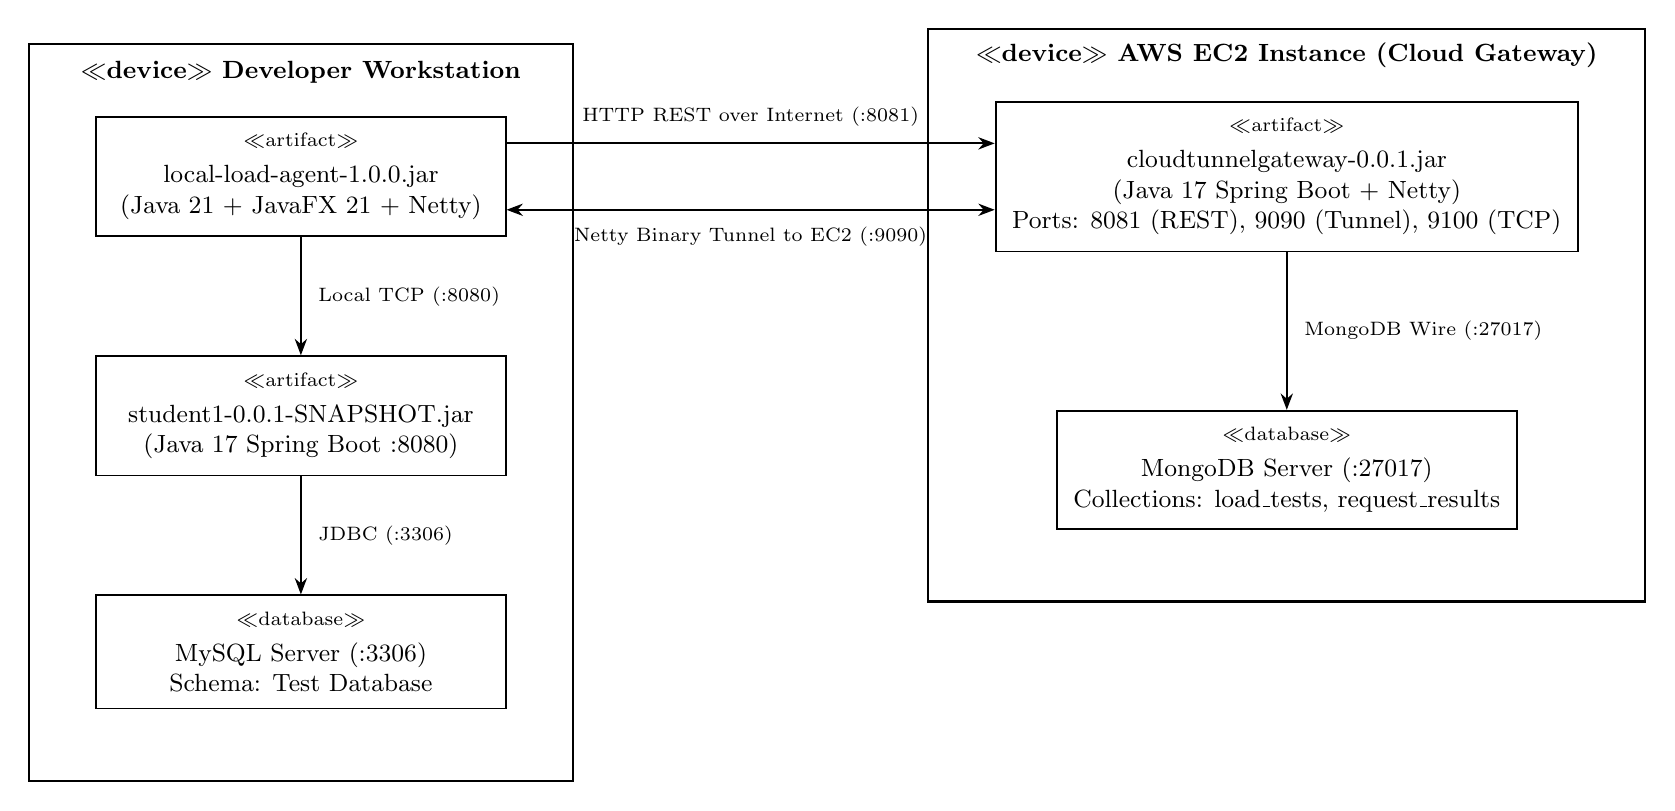
\begin{tikzpicture}[node distance=1.8cm and 4.4cm]

  % Node 1: Developer Workstation
  \node[uml box, minimum width=5.2cm] (art1) {\scriptsize$\ll$artifact$\gg$\\[2pt]\small local-load-agent-1.0.0.jar\\(Java 21 + JavaFX 21 + Netty)};
  \node[uml box, minimum width=5.2cm, below=1.5cm of art1] (art2) {\scriptsize$\ll$artifact$\gg$\\[2pt]\small student1-0.0.1-SNAPSHOT.jar\\(Java 17 Spring Boot :8080)};
  \node[uml box, minimum width=5.2cm, below=1.5cm of art2] (art3) {\scriptsize$\ll$database$\gg$\\[2pt]\small MySQL Server (:3306)\\Schema: Test Database};

  \begin{scope}[on background layer]
    \node[draw=black, line width=0.85pt, fill=white,
          fit=(art1)(art2)(art3), inner xsep=24pt, inner ysep=26pt,
          label={[font=\bfseries\small, yshift=-18pt]north:$\ll$device$\gg$ Developer Workstation}] (node1) {};
  \end{scope}

  % Node 2: Cloud / Gateway Host
  \node[uml box, minimum width=5.6cm, right=6.2cm of art1] (art4) {\scriptsize$\ll$artifact$\gg$\\[2pt]\small cloudtunnelgateway-0.0.1.jar\\(Java 17 Spring Boot + Netty)\\Ports: 8081 (REST), 9090 (Tunnel), 9100 (TCP)};
  \node[uml box, minimum width=5.6cm, below=2.0cm of art4] (art5) {\scriptsize$\ll$database$\gg$\\[2pt]\small MongoDB Server (:27017)\\Collections: load\_tests, request\_results};

  \begin{scope}[on background layer]
    \node[draw=black, line width=0.85pt, fill=white,
          fit=(art4)(art5), inner xsep=24pt, inner ysep=26pt,
          label={[font=\bfseries\small, yshift=-18pt]north:$\ll$device$\gg$ AWS EC2 Instance (Cloud Gateway)}] (node2) {};
  \end{scope}

  % Internal and cross-node communication paths
  \draw[uml arrow] (art1.south) -- node[lbl, right=4pt] {Local TCP (:8080)} (art2.north);
  \draw[uml arrow] (art2.south) -- node[lbl, right=4pt] {JDBC (:3306)} (art3.north);
  \draw[uml arrow] (art4.south) -- node[lbl, right=4pt] {MongoDB Wire (:27017)} (art5.north);

  \draw[uml arrow]   ([yshift=12pt]art1.east) -- node[lbl, above=4pt] {HTTP REST over Internet (:8081)} ([yshift=12pt]art4.west);
  \draw[uml biarrow] ([yshift=-12pt]art1.east) -- node[lbl, below=4pt] {Netty Binary Tunnel to EC2 (:9090)} ([yshift=-12pt]art4.west);

\end{tikzpicture}%
}
\caption{Deployment Diagram: Hardware/Execution Nodes, Deployed JAR Artifacts, and Network Ports.}
\label{fig:deploy}
\end{figure}

\section{Screenshots}

The screenshots below capture \texttt{LocalLoadAgent} connected to \texttt{CloudTunnelGateway} on AWS EC2 while load-testing \texttt{http://localhost:8080/api/users} on \texttt{student1}.

\begin{figure}[!htbp]
\centering
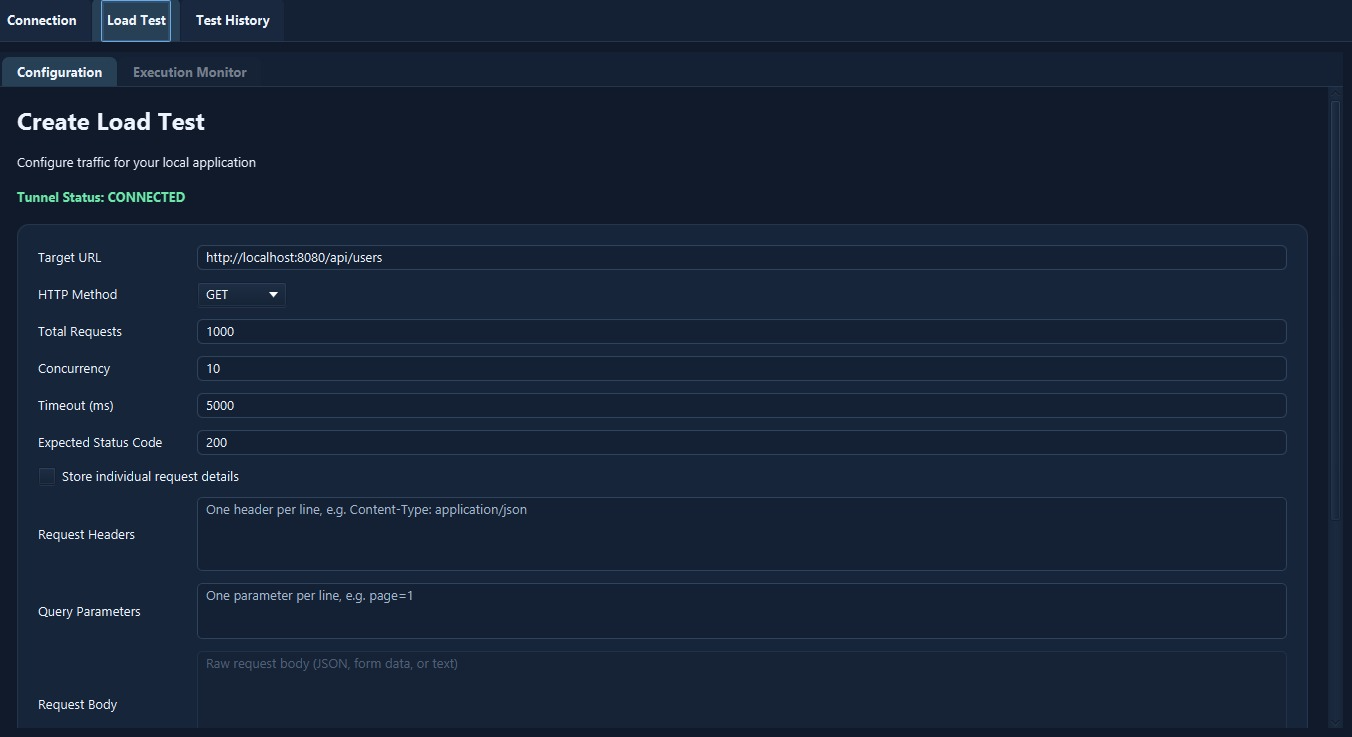
\includegraphics[width=0.84\linewidth,height=6.6cm,keepaspectratio]{screenshots/fig_4_3_1_create_load_test.png}
\caption{Load Test Configuration interface (\texttt{LoadTestView}) with active \texttt{CONNECTED} tunnel.}
\label{fig:ss1}
\end{figure}

\begin{figure}[!htbp]
\centering
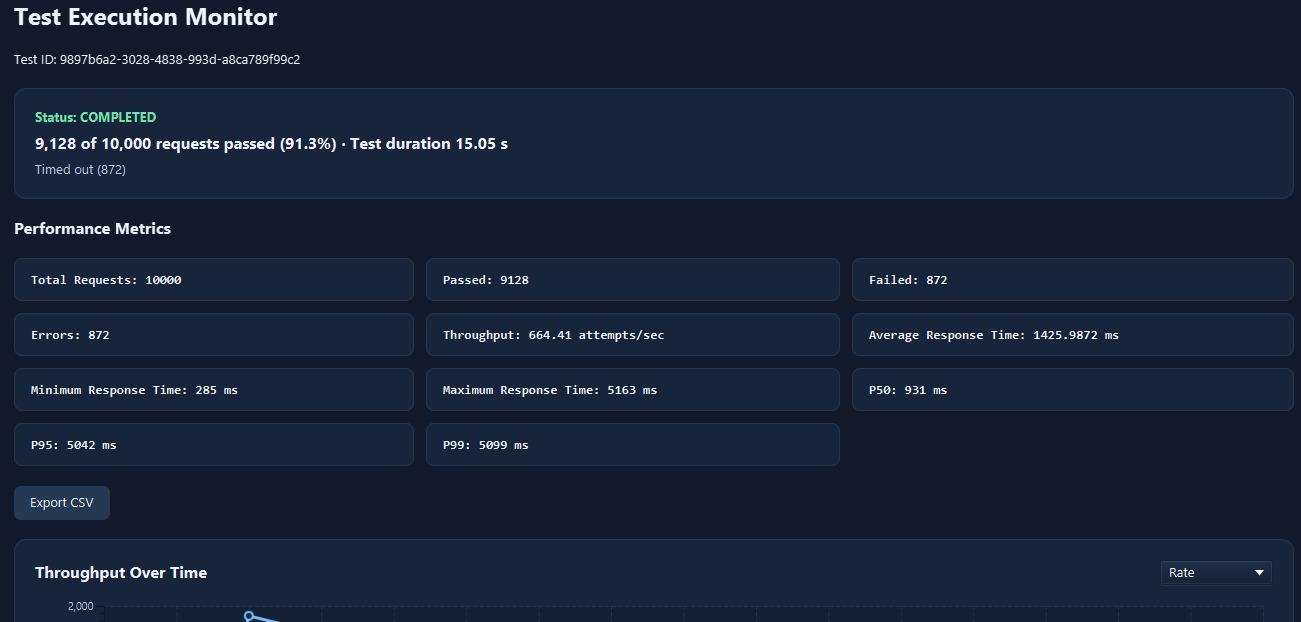
\includegraphics[width=0.84\linewidth,height=6.6cm,keepaspectratio]{screenshots/fig_4_3_2_execution_monitor.png}
\caption{Test Execution Monitor summary KPIs for a 10,000-request benchmark (Test ID \texttt{9897b6a2...}).}
\label{fig:ss2}
\end{figure}

\begin{figure}[!htbp]
\centering
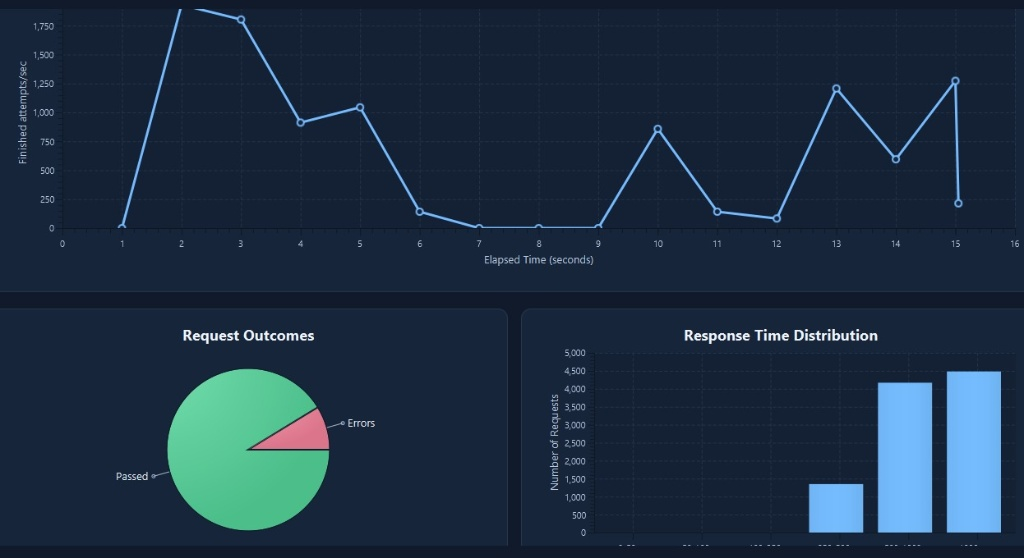
\includegraphics[width=0.84\linewidth,height=6.6cm,keepaspectratio]{screenshots/fig_4_3_4_outcomes_and_distribution.jpg}
\caption{Throughput Over Time, Request Outcomes pie chart, and Response Time Distribution bar chart.}
\label{fig:ss3}
\end{figure}

\begin{figure}[!htbp]
\centering
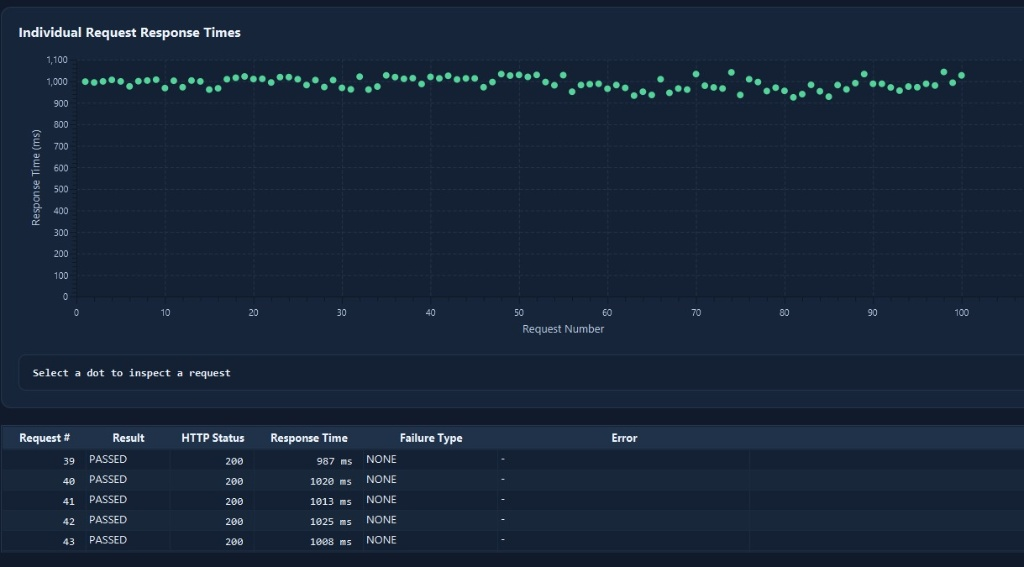
\includegraphics[width=0.84\linewidth,height=6.6cm,keepaspectratio]{screenshots/fig_4_3_5_scatter_and_requests.jpg}
\caption{Individual Request Response Times scatter plot and paginated request inspection table.}
\label{fig:ss4}
\end{figure}

\begin{figure}[!htbp]
\centering
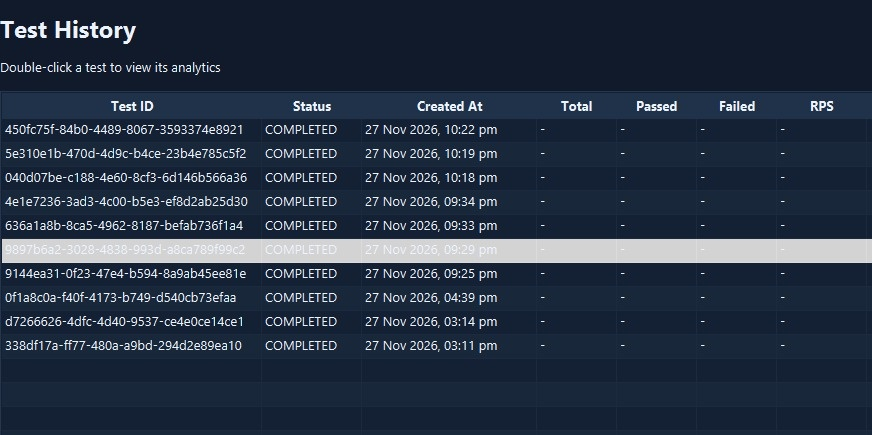
\includegraphics[width=0.84\linewidth,height=6.6cm,keepaspectratio]{screenshots/fig_4_3_6_test_history.jpg}
\caption{Test History view (\texttt{TestHistoryView}) displaying persisted MongoDB test runs.}
\label{fig:ss5}
\end{figure}

% =====================================================================
% CHAPTER 5: TESTING
% =====================================================================
\chapter{Testing}

\section{Test Plan}

Testing verified functional correctness, AWS EC2 reverse-tunnel stability, assertion accuracy, high-concurrency load execution, persistence, and UI responsiveness across all three Maven modules. Automated JUnit 5 tests validated \texttt{student1} against an embedded H2 database in MySQL mode, while end-to-end benchmarks ran against the live \textbf{AWS EC2} gateway, MongoDB, and local MySQL Test Database.

\begin{table}[!htbp]
\centering
\small
\caption{System Test Plan Matrix}
\label{tab:testplan}
\begin{tabularx}{\linewidth}{|L{2.9cm}|L{3.9cm}|Y|}
\hline
\textbf{Test Area} & \textbf{Objective} & \textbf{Approach} \\
\hline
Target Service API & Verify CRUD \& validation on \texttt{student1} & Run JUnit integration tests (\texttt{POST/GET /api/users}) with valid and blank payloads. \\
\hline
AWS EC2 Tunnel Handshake & Verify Netty registration \& status updates & Connect \texttt{LocalLoadAgent} to AWS EC2 on \texttt{:9090}; confirm \texttt{REGISTER\_ACK} and \texttt{CONNECTED} status. \\
\hline
Input Validation & Prevent invalid load-test submissions & Submit tests while disconnected, with invalid HTTP status codes ($<100$ or $>599$), or out-of-range counts. \\
\hline
Tunneled Load Execution & Verify high-concurrency stream multiplexing & Run 100-request and 10,000-request benchmarks from AWS EC2 (\texttt{:9100}) to \texttt{localhost:8080/api/users}. \\
\hline
Analytics \& Persistence & Verify MongoDB storage \& percentile math & Confirm \texttt{load\_tests} and \texttt{request\_results} documents, P50/P95/P99 values, and history pagination. \\
\hline
CSV Export & Verify offline report generation & Export completed run to CSV and inspect summary, throughput, distribution, and request rows. \\
\hline
\end{tabularx}
\end{table}

\section{Test Cases}

\begin{table}[!htbp]
\centering
\footnotesize
\caption{Functional and Performance Test Cases}
\label{tab:testcases}
\begin{tabularx}{\linewidth}{|L{1.1cm}|L{2.7cm}|Y|Y|L{1.1cm}|}
\hline
\textbf{ID} & \textbf{Scenario} & \textbf{Expected Result} & \textbf{Actual Result} & \textbf{Status} \\
\hline
TC-01 & Create users via \texttt{POST /api/users} & HTTP 201 with sequential IDs returned and readable via \texttt{GET} & Verified in JUnit tests; two users created with sequential IDs & Pass \\
\hline
TC-02 & Submit blank name to \texttt{POST /api/users} & HTTP 400 Bad Request returned & \texttt{BadRequest} exception thrown as expected & Pass \\
\hline
TC-03 & Connect agent to AWS EC2 \texttt{:9090} & \texttt{REGISTER\_ACK} received; UI shows \texttt{CONNECTED} & Tunnel registered cleanly over AWS EC2; green badge shown & Pass \\
\hline
TC-04 & Submit test while disconnected & Submission blocked with disconnected error & \texttt{LoadTestView} disabled submission and displayed error & Pass \\
\hline
TC-05 & 100-request GET load test & 100/100 routed via tunnel, HTTP 200, scatter populated & 100/100 passed (\texttt{HTTP 200}, $\sim$930--1,040\,ms, \texttt{NONE}) & Pass \\
\hline
TC-06 & 10,000-request stress test & Sustains concurrency, classifies timeouts, computes percentiles & 9,128 passed (91.3\%), 872 timed out in 15.05\,s (664.41 req/s; P50 931\,ms, P95 5042\,ms, P99 5099\,ms) & Pass \\
\hline
TC-07 & Browse \texttt{TestHistoryView} & Paginated MongoDB runs listed & 10 completed runs (27 Nov 2026) listed; double-click opened analytics & Pass \\
\hline
TC-08 & Export completed run to CSV & CSV written with summary, charts data, and requests & Export succeeded cleanly from \texttt{TestExecutionView} & Pass \\
\hline
\end{tabularx}
\end{table}

\subsection{Additional Deployment and End-to-End Checks}

\begin{table}[!htbp]
\centering
\small
\caption{AWS EC2 Deployment and End-to-End Integration Checks}
\label{tab:deploychecks}
\begin{tabularx}{\linewidth}{|L{3.7cm}|Y|}
\hline
\textbf{Check} & \textbf{Observed Result} \\
\hline
AWS EC2 Instance Hosting & Deployed the \texttt{cloudtunnelgateway} JAR on an AWS EC2 instance with inbound security-group rules configured for ports \texttt{8081}, \texttt{9090}, and \texttt{9100}. \\
\hline
Netty Tunnel Gateway (\texttt{:9090}) & Started via \texttt{GatewayStartup} on AWS EC2; accepted outbound agent registration from the local workstation and framed binary messages. \\
\hline
Public TCP Ingress (\texttt{:9100}) & Started via \texttt{PublicTcpServerStartup} on AWS EC2; multiplexed concurrent streams via \texttt{StreamRegistry}. \\
\hline
Gateway REST API (\texttt{:8081}) & Served \texttt{/api/load-tests}, \texttt{/\{testId\}}, \texttt{/results}, \texttt{/request-results}, and \texttt{/history} remotely from AWS EC2. \\
\hline
MongoDB Persistence & Stored \texttt{LoadTestDocument} in \texttt{load\_tests} and batched \texttt{RequestResultDocument} in \texttt{request\_results}. \\
\hline
MySQL Test Database & Auto-initialized \texttt{student\_test\_users} in the local Test Database (\texttt{spring.sql.init.mode=always}). \\
\hline
\end{tabularx}
\end{table}

\section{Test Reports by Peers}

Peer evaluation was conducted during live demonstrations of the AWS EC2-backed load testing workflow. Table~\ref{tab:peer_testing} summarises the feedback, observations, and corresponding resolutions.

\begin{table}[!htbp]
\centering
\small
\caption{Peer Testing Feedback}
\label{tab:peer_testing}
\begin{tabularx}{\linewidth}{|L{2.5cm}|Y|Y|Y|}
\hline
\textbf{Peer / Group} & \textbf{Feedback} & \textbf{Issue / Observation} & \textbf{Resolution} \\
\hline
Peer Group A (CSE-3Q) & Live KPI cards and throughput chart make high-load bottlenecks immediately visible. & Submitting a load test before connecting the tunnel initially caused confusion. & Added an explicit colour-coded \texttt{Tunnel Status} indicator and disabled submission when disconnected. \\
\hline
Peer Group B (CSE-3Q) & Reverse tunneling from AWS EC2 to a local Spring Boot app worked smoothly without port forwarding. & Large 10,000-request runs needed an easier way to inspect individual slow or timed-out requests. & Added paginated request tables (100 rows/page) and clickable dots on the scatter plot. \\
\hline
Peer Group C (CSE-3Q) & Test History and MongoDB persistence are useful for comparing repeated benchmarks. & Exporting raw results for external plotting was requested during the demo. & Verified one-click CSV export containing summary KPIs, throughput buckets, and request rows. \\
\hline
\end{tabularx}
\end{table}

\section{Testing Summary}

End-to-end testing confirmed that the \textit{Cloud Tunnel Gateway and Local Load Testing Platform}, with \texttt{CloudTunnelGateway} deployed on \textbf{AWS EC2}, reliably establishes outbound reverse Netty tunnels from the developer workstation, multiplexes concurrent TCP streams to the local \texttt{student1} service and MySQL Test Database, evaluates HTTP status and response assertions, and persists telemetry to MongoDB. Automated JUnit tests verified target API validation, while the 10,000-request stress benchmark sustained 664.41 attempts/sec over 15.05 seconds with accurate timeout classification (872 timeouts) and tail-latency reporting (P50: 931\,ms, P95: 5042\,ms, P99: 5099\,ms).

% =====================================================================
% BIBLIOGRAPHY
% =====================================================================
\begin{thebibliography}{9}

\bibitem{netty}
The Netty Project, \textit{Netty 4.1 User Guide and API Documentation}. Available at: \url{https://netty.io/wiki/user-guide-for-4.x.html}

\bibitem{springboot}
VMware, Inc., \textit{Spring Boot Reference Documentation}. Available at: \url{https://docs.spring.io/spring-boot/}

\bibitem{javafx}
OpenJFX Community, \textit{JavaFX 21 Documentation}. Available at: \url{https://openjfx.io/}

\bibitem{mongodb}
MongoDB, Inc., \textit{MongoDB Manual and Spring Data MongoDB}. Available at: \url{https://www.mongodb.com/docs/}

\bibitem{aws}
Amazon Web Services, \textit{Amazon EC2 Documentation}. Available at: \url{https://docs.aws.amazon.com/ec2/}

\bibitem{uml}
Object Management Group (OMG), \textit{Unified Modeling Language (UML) Version 2.5.1 Specification}. Available at: \url{https://www.uml-diagrams.org/uml-25-diagrams.html}

\end{thebibliography}

\end{document}
